\documentclass{scalatekids-article}
\begin{document}
\lfoot{Analisi dei Requisiti 1.0.0}
\newgeometry{top=3.5cm}
\begin{titlepage}
  \begin{center}
    \begin{center}
      
\includegraphics[width=10cm]{sklogo.png}
    \end{center}
    \vspace{1cm}
    \begin{Huge}
      \begin{center}
        \textbf{Analisi dei Requisiti}
      \end{center}
    \end{Huge}
    \vspace{11pt}
    \bgroup
    \def\arraystretch{1.3}
    \begin{tabular}{r|l}
      \multicolumn{2}{c}{\textbf{Informazioni sul documento}} \\
      \hline
      \setbox0=\hbox{0.0.1\unskip}\ifdim\wd0=0pt
      \\
      \else
      \textbf{Versione} & 1.0.0\\
      \fi
      \textbf{Redazione} & \multiLineCell[t]{Davide Trevisan\\Marco Boseggia\\Michael Munaro}\\
      \textbf{Verifica} & \multiLineCell[t]{Alberto De Agostini\\Giacomo Vanin}\\
      \textbf{Approvazione} & \multiLineCell[t]{Andrea Giacomo Baldan}\\
      \textbf{Uso} & Esterno\\
      \textbf{Lista di Distribuzione} & \multiLineCell[t]{ScalateKids\\Prof. Tullio Vardanega\\Prof. Riccardo Cardin}\\
    \end{tabular}
    \egroup
    \vspace{22pt}
  \end{center}
\end{titlepage}
\restoregeometry
\clearpage
\setcounter{page}{1}
\begin{flushleft}
  \vspace{0cm}
         {\large\bfseries Diario delle modifiche \par}
\end{flushleft}
\vspace{0cm}
\begin{center}
  \begin{tabular}{| l | l | l | l | p{5cm} |}
    \hline
    Versione & Autore & Ruolo & Data & Descrizione \\
    \hline
    1.0.0 & Andrea Giacomo Baldan & Responsabile & 2016-01-20 & Approvazione documento\\
    \hline
    0.4.0 & Giacomo Vanin & Verificatore & 2016-01-19 & Verifica capitolo Tracciamento\\
    \hline
    0.3.1 & Marco Boseggia & Analista & 2016-01-18 & Stesura capitolo Tracciamento\\
    \hline
    0.3.0 & Alberto De Agostini & Verificatore & 2016-01-16 & Verifica capitolo Classificazione Requisiti\\
    \hline
    0.2.3 & Michael Munaro & Analista & 2016-01-15 & Integrazione capitolo Classificazione Requisiti\\
    \hline
    0.2.1 & Marco Boseggia & Analista & 2016-01-14 & Stesura capitolo Classificazione Requisiti\\
    \hline
    0.2.2 & Davide Trevisan & Analista & 2016-01-14 & Correzione capitolo Casi d'uso\\
    \hline
    0.2.0 & Giacomo Vanin & Verificatore & 2016-01-12 & Verifica capitolo Casi d'uso\\
    \hline
    0.1.1 & Michael Munaro & Analista & 2016-01-10 & Integrazione capitolo Casi d'uso\\
    \hline
    0.1.0 & Alberto De Agostini & Verificatore & 2016-01-07 & Verifica capitoli stesi in precedenza\\
    \hline
    0.0.4 & Davide Trevisan & Analista & 2016-01-05 & Integrazione capitolo Casi d'uso\\
    \hline
    0.0.3 & Marco Boseggia & Analista & 2016-01-04 & Inizio stesura capitolo Casi d'uso\\
    \hline
    0.0.2 & Michael Munaro & Analista & 2016-01-03 & Stesura capitolo Descrizione Generale\\
    \hline
    0.0.1 & Andrea Giacomo Baldan & Amministratore & 2015-12-16 & Creazione scheletro del documento\\
    \hline
  \end{tabular}
\end{center}
\tableofcontents
\listoftables
\listoffigures
\newpage
\pagenumbering{arabic}
\section{Sommario}
\subsection{Scopo del documento}
Il seguente documento ha lo scopo di presentare le funzionalità che il prodotto
\textbf{Actorbase} esporrà all'utilizzatore finale. Inoltre elenca e descrive i
requisiti derivanti dalle suddette funzionalità, emersi durante le riunioni
interne ed esterne con il \textit{Proponente}.
\prodPurpose \glossExpl
\subsection{Riferimenti}
\subsubsection{Normativi}
\begin{itemize}
\item\textbf{Capitolato d'appalto C1:} \textit{Actorbase: a NoSQL DB based on the Actor model}\\
  \url{http://www.math.unipd.it/~tullio/IS-1/2015/Progetto/C1.pdf}
\item\textbf{Verbale esterno:}\\
  \href{run:VerbaleEsterno20160112\_v1.0.0.pdf}{Verbale Esterno 20160112 v1.0.0}\\
  \href{run:VerbaleEsterno20160119\_v1.0.0.pdf}{Verbale Esterno 20160119 v1.0.0}
\item\textbf{Norme di Progetto:}\\
  \href{run:../Interni/NormeDiProgetto\_v1.0.0.pdf}{Norme di Progetto v1.0.0}
\end{itemize}
\subsubsection{Informativi}
\begin{itemize}
\item\textbf{Dispense fornite dall'insegnamento Ingegneria del Software mod. A:}\\
  \url{http://www.math.unipd.it/~tullio/IS-1/2015/Dispense/L06.pdf}
\item\textbf{Dispense fornite dall'insegnamento Ingegneria del Software mod. A:}\\
  \url{http://www.math.unipd.it/~tullio/IS-1/2015/Dispense/E02.pdf}
\item\textbf{CAP theorem:}\\
  \url{https://en.wikipedia.org/wiki/CAP_theorem}
\item\textbf{Reactive Manifesto:}\\
  \url{http://www.reactivemanifesto.org/}\\
  \url{https://en.wikipedia.org/wiki/Reactive_programming}
\item\textbf{Amazon DynamoDB:}\\
  \url{http://docs.aws.amazon.com/amazondynamodb/latest/developerguide/Introduction.html}
\item\textbf{Leader election:}\\
  \url{https://en.wikipedia.org/wiki/Leader_election}
\end{itemize}
\section{Descrizione generale}
\subsection{Prospettive del prodotto}
l'obiettivo del prodotto è fornire un \gloss{database} \gloss{NoSQL} di tipo
\gloss{key-value}, quindi senza schemi predefiniti e tabelle; che utilizzi il
modello ad \gloss{attori} per garantire un alto grado di \gloss{concorrenza} e
\gloss{scalabilità orizzontale} idealmente illimitata.
\subsection{Funzioni}
Il software fornirà un sistema di interazione con l'utente basata su \gloss{UI}
testuale direttamente da riga di comando. Questa permetterà di effettuare le operazioni
basilari che ogni \gloss{database} fornisce:
\begin{itemize}
\item Creazione di una o più \gloss{collezioni};
\item Cancellazione di una o più \gloss{collezioni};
\item Modifica del nome di una \gloss{collezione};
\item Ricerca all'interno del \gloss{database} o all'interno di una o più \gloss{collezioni};
\item Inserimento \gloss{item} con o senza sovrascrittura;
\item Cancellazione \gloss{item};
\item Connessione ad altre istanze \textbf{Actorbase}.
\end{itemize}
Il programma inoltre permetterà la richiesta di un aiuto esplicativo sull'uso
dei comandi.
\subsection{Caratteristiche utenza}
Il prodotto è orientato all'utilizzo da parte di clientela interessata a
sviluppo di applicazioni \gloss{reactive}, che trattino grandi moli di dati e
debbano fornire brevissimi tempi di risposta sacrificando dunque le
funzionalità relazionali tipiche dei tradizionali \gloss{database} \textit{SQL} in
favore di un sistema fortemente \gloss{concorrente} e senza l'\gloss{overhead} generato
dagli schemi \gloss{SQL}.
\subsection{Vincoli}
Per far funzionare \textbf{Actorbase} sarà necessario disporre di un computer con
installata la \textit{\gloss{JVM} versione 8}. Non ci sono ulteriori richieste hardware o software.
\section{Casi d'uso}
Le aspettative di esperienza utente derivano dall'utilizzo da parte dei
componenti del gruppo di \gloss{Amazon DynamoDB}, un \gloss{database} \gloss{key-value}
sviluppato da \textit{Amazon}, utilizzato come modello di riferimento per lo sviluppo. I casi d'uso seguono le norme di stesura elencate nel documento \href{run:../Interni/NormeDiProgetto\_v1.0.0.pdf}{Norme di Progetto v1.0.0}.
\subsection{Identificazione attori}
L'analisi del capitolato e le riunioni con il \textit{Proponente} hanno fatto emergere
alcune considerazioni sull'obiettivo che \textbf{Actorbase} si pone di raggiungere.
Trattandosi di un'applicazione distribuita il prodotto finale sarà costituito
da due macro componenti: un lato server e un lato client fornito di interfaccia
comandi testuale per poter dialogare con la base di dati.\\ In particolare la
scalabilità che il prodotto deve fornire ha portato alla suddivisione degli
attori primari nel modo seguente:\\
\begin{itemize}
\item\textbf{Utente non autenticato:}\\
  Rappresenta l'utente generico che avvia la \gloss{CLI} di \textbf{Actorbase} ma non è ancora connesso al lato server del prodotto;
\item\textbf{Utente autenticato:}\\
  Rappresenta l'utente generico connesso al lato server del prodotto;
\item\textbf{Amministratore:}\\
  Rappresenta un superutente con privilegi di \gloss{visibilità} maggiori rispetto a utenti generici e poteri di modifica sulla \gloss{visibilità} di questi ultimi.
\end{itemize}
\subsubsection{Visibilità}
Rispetto al classico sistema di permessi di lettura e scrittura, \textbf{Actorbase}
prevede un meccanismo semplificato di \gloss{visibilità} secondo le seguenti regole:
\begin{itemize}
\item Ogni utente generico inizialmente ha \gloss{visibilità} solo sulle proprie \gloss{collezioni} e/o su \gloss{collezioni} di proprietà altrui su cui è in collaborazione;
\item L'utente amministratore ha \gloss{visibilità} su tutto il sistema \textbf{Actorbase}.
\end{itemize}
La \gloss{visibilità} garantisce privilegi sia in lettura che in scrittura. Di
conseguenza tutte le azioni descritte nei casi d'uso si applicano al livello di
\gloss{visibilità} proprio dell'attore che le effettua.
\subsubsection{Scalabilità orizzontale}
Il vantaggio più grande che il prodotto dovrà offrire sarà la possibilità di
\gloss{scale out} semplificata al massimo. Dovrà quindi essere possibile
aggiungere potenza di calcolo e capacità di carico mediante affiancamento di
macchine aggiuntive. I dati contenuti all'interno della base di dati originaria
dovranno essere redistribuiti e bilanciati tra i nuovi nodi inseriti. In questo
modo è idealmente possibile ottenere infinita capacità di carico semplicemente
aggiungendo risorse hardware qualora necessario.
\begin{figure}[H]
  \begin{center}
    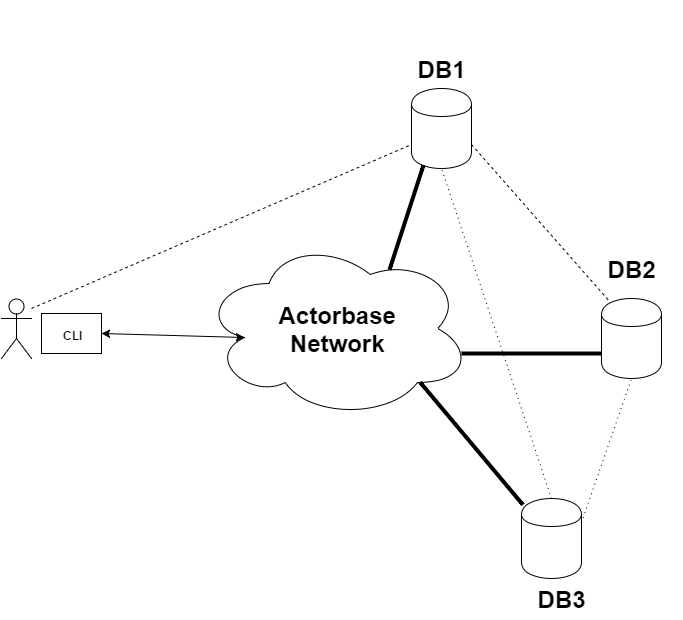
\includegraphics[width=0.7\textwidth,keepaspectratio]{UseCases/ActorbaseNetwork.png}
    \caption{Actorbase: Visione generale semplificata rete Actorbase}
  \end{center}
\end{figure}
\subsection{UC1: Actorbase}
\begin{figure}[H]
  \begin{center}
    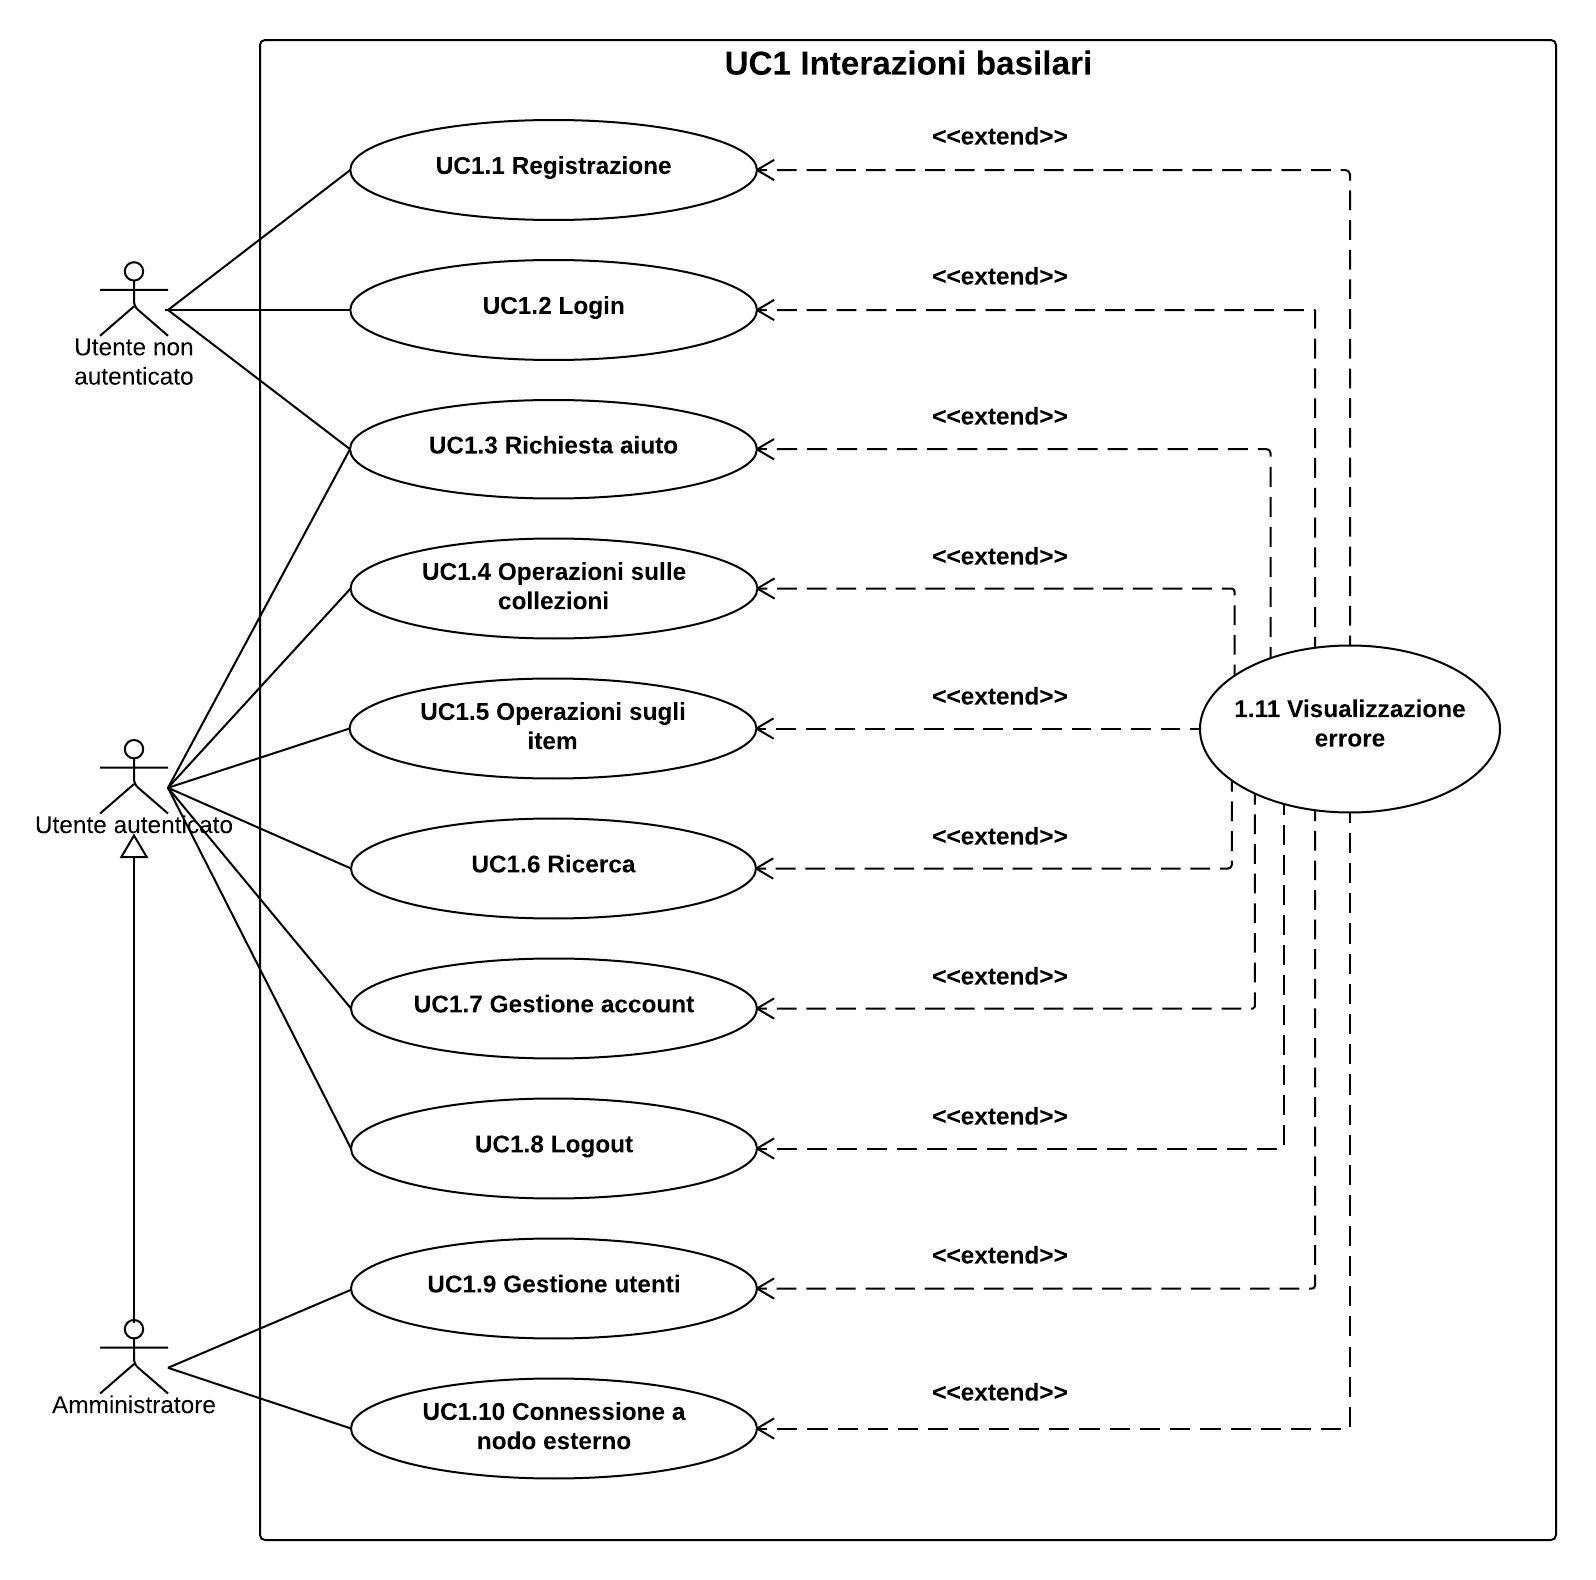
\includegraphics[width=0.7\textwidth,keepaspectratio]{UseCases/UC1.jpeg}
    \caption{Caso d'uso 1: Interazioni basilari}
  \end{center}
\end{figure}
\textbf{Attori primari:} Utente non autenticato, Utente autenticato, Amministratore\\ \\
\textbf{Scopo e descrizione:}
L’utente ha appena avviato la \gloss{CLI}, risulta essere non autenticato e può quindi
registrarsi oppure, se è già registrato, può effettuare il login diventando utente
autenticato. Le operazioni che l'utente può eseguire a login effettuato sono:
\begin{itemize}
\item Gestire il proprio \gloss{account};
\item Operazioni sulle \gloss{collezioni};
\item Operazioni sugli \gloss{item};
\item Ricerca;
\item Richiedere aiuto;
\item Effettuare il logout.
\end{itemize}
Nel caso in cui si tratti di un amministratore, oltre alle operazioni elencate, l'utente può effettuare operazioni di gestione sugli utenti
esistenti nel \gloss{database}.\\ \\
\textbf{Precondizione:} Il \gloss{database} è installato correttamente e il server è in ascolto.\\ \\
\textbf{Flusso eventi:}
\begin{itemize}
\item UC1.1 Registrazione;
\item UC1.2 Login;
\item UC1.3 Richiesta di aiuto;
\item UC1.3 Operazioni sulle \gloss{collezioni};
\item UC1.4 Operazioni sugli \gloss{item};
\item UC1.5 Ricerca;
\item UC1.6 Gestione \gloss{account};
\item UC1.7 Effettuare il logout;
\item UC1.8 Gestione utenti;
\item UC1.9 Connessione a \gloss{nodo} esterno.
\end{itemize}
\textbf{Postcondizione:} Il sistema ha prodotto l'output corrispondente al comando immesso dall'utente.
\subsection{UC1.1: Registrazione}
\textbf{Attore primario:} Utente non autenticato\\ \\
\textbf{Scopo e descrizione:} L'utente intende accedere al sistema \textbf{Actorbase}. Per farlo deve registrarsi nel sistema.
Per la registrazione è necessario inserire un nome utente e una password.\\ \\
\textbf{Precondizione:} L'utente non è registrato e richiede la registrazione.\\ \\
\textbf{Flusso eventi:}
\begin{itemize}
\item Inserimento username;
\item Inserimento password;
\item Conferma password.
\end{itemize}
\textbf{Estensioni:}
\begin{itemize}
\item Nel caso in cui l'utente utilizzi un comando sconosciuto:
  \begin{itemize}
  \item viene visualizzato un messaggio di errore esplicativo (e rimando all'aiuto).
  \end{itemize}
\item Nel caso in cui l'utente utilizzi un comando conosciuto ma con parametri errati:
  \begin{itemize}
  \item viene visualizzato un messaggio di supporto che indica come usare correttamente il comando.
  \end{itemize}
\item Nel caso in cui lo username inserito sia già presente all'interno del sistema:
  \begin{itemize}
  \item viene visualizzato un messaggio di errore esplicativo.
  \end{itemize}
\end{itemize}
\textbf{Postcondizione:} L'utente è registrato all'interno del sistema \textbf{Actorbase}.
\subsection{UC1.2: Login}
\textbf{Attore primario:} Utente non autenticato\\ \\
\textbf{Scopo e descrizione:} L’utente, già registrato, intende accedere al sistema \textbf{Actorbase}. Deve inserire le proprie credenziali di accesso. \\ \\
\textbf{Flusso di eventi:}
\begin{itemize}
\item Inserimento username;
\item Inserimento password.
\end{itemize}
\textbf{Estensioni:}
\begin{itemize}
\item Nel caso in cui l'utente utilizzi un comando sconosciuto:
  \begin{itemize}
  \item viene visualizzato un messaggio di errore esplicativo (e rimando all'aiuto).
  \end{itemize}
\item Nel caso in cui l'utente utilizzi un comando conosciuto ma con parametri errati:
  \begin{itemize}
  \item viene visualizzato un messaggio di supporto che indica come usare correttamente il comando.
  \end{itemize}
\end{itemize}
\textbf{Postcondizione:} L'utente è autenticato all'interno del sistema \textbf{Actorbase}.
\subsection{UC1.3: Richiesta aiuto}
\begin{figure}[H]
  \begin{center}
    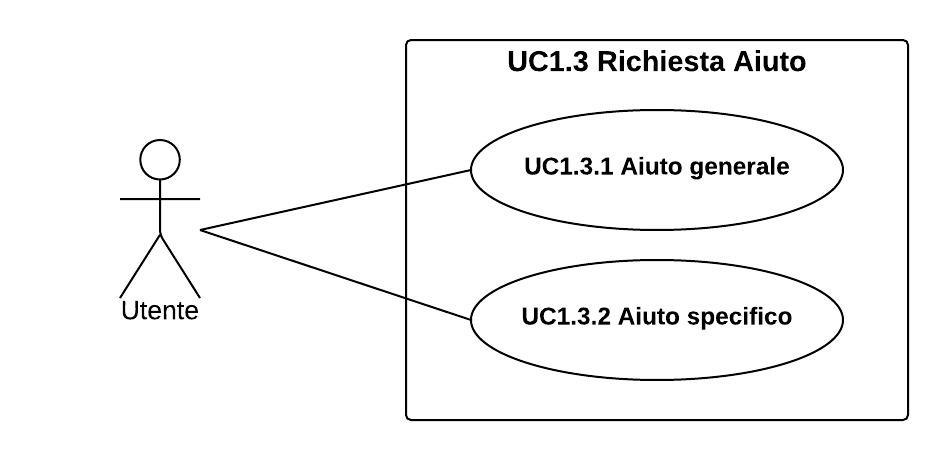
\includegraphics[width=0.7\textwidth,keepaspectratio]{UseCases/UC1_3.jpeg}
    \caption{Caso d'uso 1.3: Richiesta aiuto}
  \end{center}
\end{figure}
\textbf{Attore primario:} Utente\\ \\
\textbf{Scopo e descrizione:} L'utente intende richiedere aiuto generale o su un comando specifico.\\Nel caso di richiesta di aiuto generale diversi tipi di utente riceveranno la lista dei comandi da loro eseguibili\\ \\
\textbf{Precondizione:} Il database è pronto a ricevere comandi e l'utente intende richiedere supporto.\\ \\
\textbf{Flusso di eventi:}
\begin{itemize}
\item UC1.3.1 Inserimento comando per richiesta di aiuto generale;
\item UC1.3.2 Inserimento comando per richiesta di aiuto specifico.
\end{itemize}
\textbf{Postcondizione:} Il sistema ha risposto producendo in output l'aiuto richiesto.
\subsection{UC1.3.1: Richiesta di aiuto generale}
\textbf{Attore primario:} Utente\\ \\
\textbf{Scopo e descrizione:} L'utente intende richiedere aiuto generale sull'utilizzo del sistema \textbf{Actorbase}.\\ \\
\textbf{Precondizione:} Il \gloss{database} è pronto a ricevere comandi e l'utente intende richiedere supporto.\\ \\
\textbf{Flusso di eventi:}
\begin{itemize}
\item Inserimento comando per richiesta di aiuto.
\end{itemize}
\textbf{Postcondizione:} Il sistema ha risposto visualizzando l'aiuto richiesto dall'utente in output.
\subsection{UC1.3.2: Richiesta di aiuto specifico}
\textbf{Attore primario:} Utente\\ \\
\textbf{Scopo e descrizione:} L'utente intende richiedere aiuto su uno specifico comando del sistema \textbf{Actorbase}.\\ \\
\textbf{Flusso di eventi:}
\begin{itemize}
\item inserimento comando per richiesta di aiuto;
\item Inserimento nome comando.
\end{itemize}
\textbf{Postcondizione:} Il sistema ha risposto visualizzando l'aiuto richiesto dall'utente in output.
\subsection{UC1.4: Operazioni sulle collezioni}
\begin{figure}[H]
  \begin{center}
    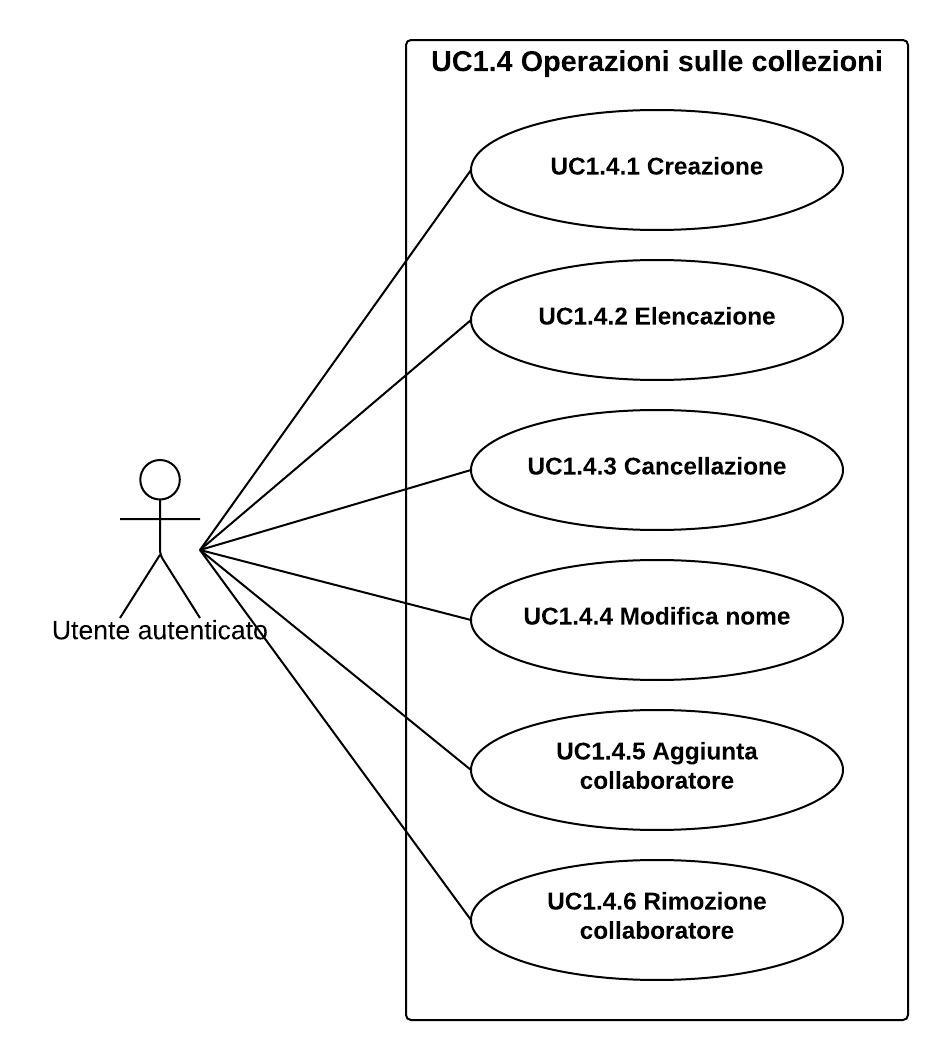
\includegraphics[width=0.7\textwidth,keepaspectratio]{UseCases/UC1_4.jpeg}
    \caption{Caso d'uso 1.4: Operazioni sulle \gloss{collezioni}}
  \end{center}
\end{figure}
\textbf{Attore primario:} Utente autenticato\\ \\
\textbf{Scopo e descrizione:} L'utente è autenticato e desidera effettuare delle operazioni sulle \gloss{collezioni}. Le operazioni previste sono:
creazione di una nuova \gloss{collezione}, elencazione delle \gloss{collezioni} esistenti, cancellazione di \gloss{collezioni} esistenti, modifica del nome di \gloss{collezioni} esistenti e
aggiunta o rimozione collaboratori a \gloss{collezione} esistente.\\ \\
\textbf{Precodizione:} Il \gloss{database} è pronto a ricevere comandi e l'utente intende effettuare operazioni su \gloss{collezioni}.\\ \\
\textbf{Flusso di eventi:}
\begin{itemize}
\item UC1.4.1 Creazione nuova \gloss{collezione};
\item UC1.4.2 Elencazione \gloss{collezioni};
\item UC1.4.3 Cancellazione \gloss{collezioni};
\item UC1.4.6 Modifica nome \gloss{collezione};
\item UC1.4.4 Aggiunta collaboratore;
\item UC1.4.5 Rimozione collaboratore.
\end{itemize}
\textbf{Estensioni:}
\begin{itemize}
\item Nel caso in cui l'utente utilizzi un comando sconosciuto:
  \begin{itemize}
  \item viene visualizzato un messaggio di errore esplicativo (e rimando all'aiuto).
  \end{itemize}
\item Nel caso in cui l'utente utilizzi un comando conosciuto ma con parametri errati:
  \begin{itemize}
  \item viene visualizzato un messaggio di supporto che indica come usare correttamente il comando.
  \end{itemize}
\item Nel caso in cui il nome di una \gloss{collezione} sia già utilizzato:
  \begin{itemize}
  \item viene visualizzato un messaggio di errore esplicativo.
  \end{itemize}
\item Nel caso in cui la \gloss{collezione} da cancellare o modificare non sia presente:
  \begin{itemize}
  \item viene visualizzato un messaggio di errore esplicativo.
  \end{itemize}
\item Nel caso in cui il collaboratore da rimuovere non sia presente tra i collaboratori:
  \begin{itemize}
  \item viene visualizzato un messaggio di errore esplicativo.
  \end{itemize}
\item Nel caso in cui il collaboratore da aggiungere non sia presente nel sistema \textbf{Actorbase}:
  \begin{itemize}
  \item viene visualizzato un messaggio di errore esplicativo.
  \end{itemize}
\end{itemize}
\textbf{Postcondizione:} L'operazione richiesta è stata eseguita.
\subsection{UC1.4.1: Creazione nuova collezione}
\textbf{Attore primario:} Utente autenticato\\ \\
\textbf{Scopo e descrizione:} L'utente richiede la creazione di una \gloss{collezione} all'interno del \gloss{database}, deve inserire il nome della nuova \gloss{collezione}.\\ \\
\textbf{Precodizione:} Il \gloss{database} è pronto a ricevere comandi e l'utente intende creare una \gloss{collezione}.\\ \\
\textbf{Flusso di eventi:}
\begin{itemize}
\item Inserimento nome \gloss{collezione}
\end{itemize}
\textbf{Postcondizione:} La \gloss{collezione} è stata creata.
\subsection{UC1.4.2: Elencazione collezioni}
\textbf{Attore primario:} Utente autenticato\\ \\
\textbf{Scopo e descrizione:} L'utente intende elencare tutte le \gloss{collezioni} all'interno di \textbf{Actorbase} secondo la propria \gloss{visibilità}.\\ \\
\textbf{Precodizione:} Il \gloss{database} è pronto a ricevere comandi e l'utente intende elencare le \gloss{collezioni} al suo interno.\\ \\
\textbf{Postcondizione:} Il \gloss{database} restituisce la lista delle \gloss{collezioni} esistenti secondo la \gloss{visibilità} dell'utente.
\subsection{UC1.4.3: Cancellazione di una o più collezioni}
\textbf{Attore primario:} Utente autenticato\\ \\
\textbf{Scopo e descrizione:} L’utente intende cancellare una o più \gloss{collezioni} presenti nel \gloss{database}.\\ \\
\textbf{Precodizione:} Il \gloss{database} è pronto a ricevere comandi e l’utente intende cancellare una o più \gloss{collezioni}.\\ \\
\textbf{Flusso di eventi:}
\begin{itemize}
\item Inserimento di uno o più nomi di \gloss{collezioni} da cancellare.
\end{itemize}
\textbf{Postcondizione:} Le \gloss{collezioni} sono state rimosse dal \gloss{database}.
\subsection{UC1.4.4: Modifica nome collezione}
\textbf{Attore primario:} Utente autenticato \\ \\
\textbf{Scopo e descrizione:} L’utente intende modificare il nome di una \gloss{collezione}, deve inserire il nome della \gloss{collezione} da modificare e il nuovo nome da assegnare. \\ \\
\textbf{Precondizione:} Il \gloss{database} è pronto a ricevere comandi e l’utente intende modificare il nome di una \gloss{collezione}.\\ \\
\textbf{Flusso di eventi:}
\begin{itemize}
\item Inserimento nome della \gloss{collezione} da modificare;
\item Inserimento nuovo nome della \gloss{collezione}.
\end{itemize}
\textbf{Postcondizione:} Il nome della \gloss{collezione} è stato modificato.
\subsection{UC1.4.5: Aggiunta di un collaboratore a propria collezione}
\textbf{Attore primario:} Utente autenticato\\ \\
\textbf{Scopo e descrizione:} L'utente intende aggiungere un \gloss{collaboratore} ad una \gloss{collezione} di sua proprietà. Deve inserire il nome della \gloss{collezione} e lo username dell'utente da aggiungere.\\ \\
\textbf{Precondizione:} Il \gloss{database} è pronto a ricevere comandi e l'utente intende aggiungere un \gloss{collaboratore} ad una \gloss{collezione} di sua proprietà.\\ \\
\textbf{Flusso di eventi:}
\begin{itemize}
\item Inserimento nome \gloss{collezione};
\item Inserimento username \gloss{collaboratore}.
\end{itemize}
\textbf{Postcondizione:} L'utente designato per la collaborazione è stato aggiunto tra i \gloss{collaboratori} della \gloss{collezione} scelta.
\subsection{UC1.4.6: Rimozione di un collaboratore a propria collezione}
\textbf{Attore primario:} Utente autenticato\\ \\
\textbf{Scopo e descrizione:} L'utente intende rimuovere un \gloss{collaboratore} da una \gloss{collezione} di sua proprietà. Deve inserire il nome della \gloss{collezione} e lo username del \gloss{collaboratore} da rimuovere.\\ \\
\textbf{Precondizione:} Il \gloss{database} è pronto a ricevere comandi e l'utente intende rimuovere un \gloss{collaboratore} da una \gloss{collezione} di sua proprietà.\\ \\
\textbf{Flusso di eventi:}
\begin{itemize}
\item Inserimento nome \gloss{collezione};
\item Inserimento username \gloss{collaboratore}.
\end{itemize}
\textbf{Postcondizione:} L'utente designato per la rimozione dai \gloss{collaboratori} è stato rimosso dalla \gloss{collezione} scelta.
\subsection{UC1.5: Operazioni sugli item}
\begin{figure}[H]
  \begin{center}
    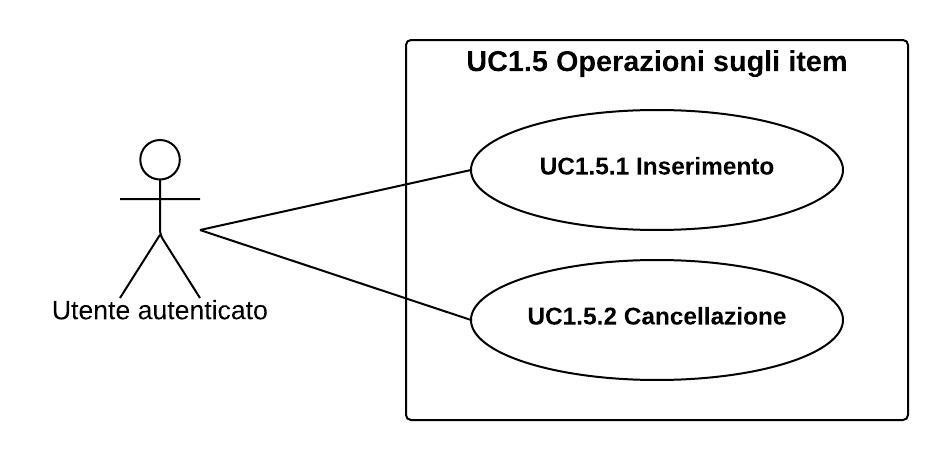
\includegraphics[width=0.7\textwidth,keepaspectratio]{UseCases/UC1_5.jpeg}
    \caption{Caso d'uso 1.5: Operazioni sugli \gloss{item}}
  \end{center}
\end{figure}
\textbf{Attore primario:} Utente autenticato\\ \\
\textbf{Scopo e descrizione:} L'utente intende effettuare operazioni sugli \gloss{item} di una \gloss{collezione} esistente. Le operazioni previste sono:
inserimento e cancellazione.\\ \\
\textbf{Precondizione:} Il \gloss{database} è pronto a ricevere comandi e l'utente intende effettuare operazioni di inserimento o cancellazione su una \gloss{collezione} esistente.\\ \\
\textbf{Flusso di eventi:}
\begin{itemize}
\item UC1.5.1 Inserimento nuovo \gloss{item};
\item UC1.5.2 Cancellazione \gloss{item}.
\end{itemize}
\textbf{Estensioni:}
\begin{itemize}
\item Nel caso in cui l'utente utilizzi un comando sconosciuto:
  \begin{itemize}
  \item viene visualizzato un messaggio di errore esplicativo (e rimando all'aiuto).
  \end{itemize}
\item Nel caso in cui l'utente utilizzi un comando conosciuto ma con parametri errati:
  \begin{itemize}
  \item viene visualizzato un messaggio di supporto che indica come usare correttamente il comando.
  \end{itemize}
\item Nel caso in cui la \gloss{collezione} su cui effettuare inserimento o cancellazione non sia presente:
  \begin{itemize}
  \item viene visualizzato un messaggio di errore esplicativo.
  \end{itemize}
\item Nel caso in cui l'\gloss{item} da rimuovere non sia presente:
  \begin{itemize}
  \item viene visualizzato un messaggio di errore esplicativo.
  \end{itemize}
\end{itemize}
\textbf{Postcondizione:} L'operazione richiesta è stata effettuata correttamente.
\subsection{UC1.5.1: Inserimento nuovo item}
\begin{figure}[H]
  \begin{center}
    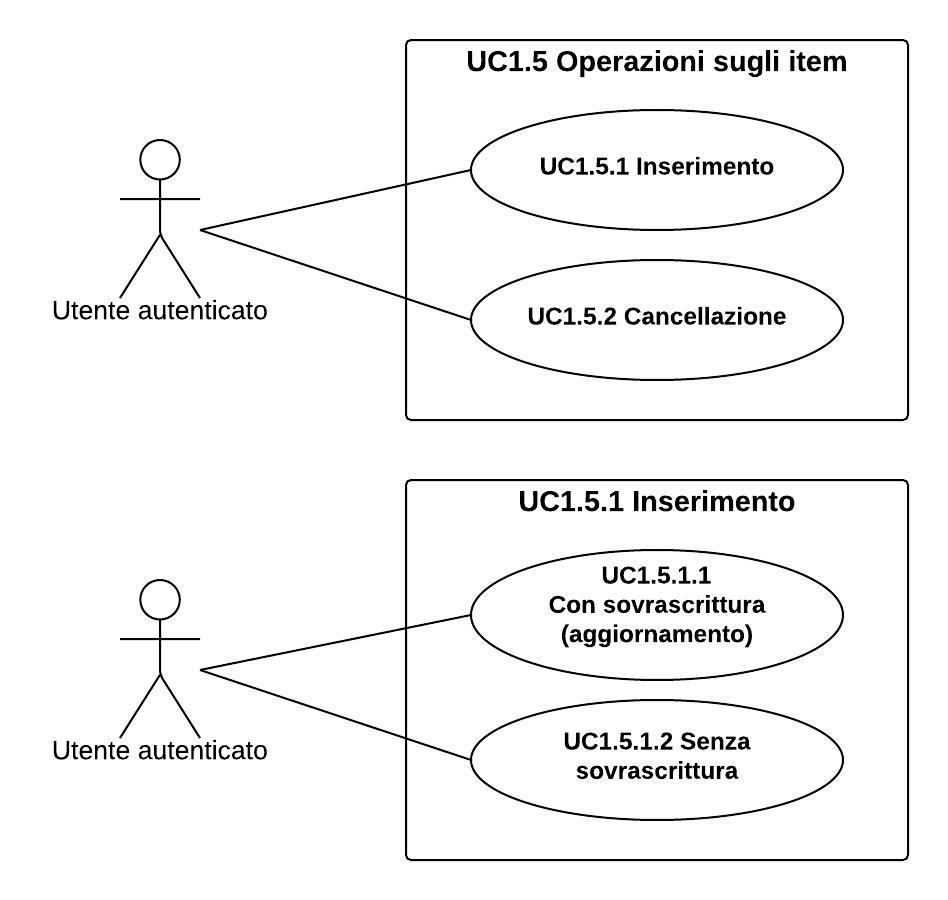
\includegraphics[width=0.7\textwidth,keepaspectratio]{UseCases/UC1_5_1.jpeg}
    \caption{Caso d'uso 1.5.1: Inserimento nuovo \gloss{item}}
  \end{center}
\end{figure}
\textbf{Attore primario:} Utente autenticato\\ \\
\textbf{Scopo e descrizione:} L'utente intende inserire un nuovo \gloss{item} all'interno di una \gloss{collezione} esistente. Deve selezionare la \gloss{collezione} e inserire i parametri di definizione dell'\gloss{item}. Questi sono la chiave e il valore associato.\\ \\
\textbf{Precondizione:} Il \gloss{database} è pronto a ricevere comandi e l'utente intende effettuare un inserimento di un nuovo \gloss{item}.\\ \\
\textbf{Flusso di eventi:}
\begin{itemize}
\item UC1.5.1.1 Inserimento con sovrascrittura;
\item UC1.5.1.2 Inserimento senza sovrascrittura.
\end{itemize}
\textbf{Postcondizione:} L'operazione di inserimento richiesta è stata effettuata correttamente.
\subsection{UC1.5.1.1: Inserimento con sovrascrittura (aggiornamento)}
\textbf{Attore primario:} Utente autenticato\\ \\
\textbf{Scopo e descrizione:} L'utente intende inserire un nuovo \gloss{item}; deve selezionare la \gloss{collezione} e inserire i parametri di definizione dell'\gloss{item} da inserire, quali chiave e valore associato. La procedura di inserimento non terrà conto di
eventuali chiavi già presenti all'interno della \gloss{collezione}\\ \\
\textbf{Precondizione:} Il \gloss{database} è pronto a ricevere comandi e l'utente intende effettuare un inserimento di un nuovo \gloss{item}.\\ \\
\textbf{Flusso di eventi:}
\begin{itemize}
\item Inserimento nome \gloss{collezione} su cui effettuare l'inserimento;
\item Inserimento coppia chiave-valore da inserire.
\end{itemize}
\textbf{Postcondizione:} L'operazione di inserimento con sovrascrittura è andata a buon fine, eventuali chiavi già presenti avranno i valori associati aggiornati.
\subsection{UC1.5.1.2: Inserimento senza sovrascrittura}
\textbf{Attore primario:} Utente autenticato \\ \\
\textbf{Scopo e descrizione:} L'utente intende inserire un nuovo \gloss{item}; deve selezionare la \gloss{collezione} e inserire i parametri di definizione dell'\gloss{item} da inserire, quali chiave e valore associato. La procedura di inserimento terrà conto di chiavi già presenti all'interno della \gloss{collezione} selezionata.\\ \\
\textbf{Precondizione:} Il \gloss{database} è pronto a ricevere comandi e l'utente intende effettuare un inserimento di un nuovo \gloss{item}.\\ \\
\textbf{Flusso di eventi:}
\begin{itemize}
\item Inserimento nome \gloss{collezione} su cui effettuare l'inserimento;
\item Inserimento coppia chiave-valore da inserire.
\end{itemize}
\textbf{Estensioni:}
\begin{itemize}
\item Nel caso in cui la chiave scelta sia già presente all'interno della \gloss{collezione}:
  \begin{itemize}
  \item viene visualizzato un messaggio di errore esplicativo;
  \end{itemize}
\end{itemize}
\textbf{Postcondizione:} L'operazione di inserimento senza sovrascrittura è andata a buon fine.
\subsection{UC1.5.2: Cancellazione di un item}
\textbf{Attore primario:} Utente autenticato\\ \\
\textbf{Scopo e descrizione:} L'utente intende cancellare un \gloss{item} all'interno di una \gloss{collezione} esistente. Deve selezionare la \gloss{collezione} e inserire la chiave del valore da cancellare.\\ \\
\textbf{Precondizione:} Il \gloss{database} è pronto a ricevere comandi e l'utente intende effettuare la cancellazione di un \gloss{item}.\\ \\
\textbf{Flusso di eventi:}
\begin{itemize}
\item Inserimento nome \gloss{collezione};
\item Inserimento chiave.
\end{itemize}
\textbf{Postcondizione:} L'operazione di cancellazione di un \gloss{item} è andata a buon fine.
\subsection{UC1.6: Ricerca generale}
\begin{figure}[H]
  \begin{center}
    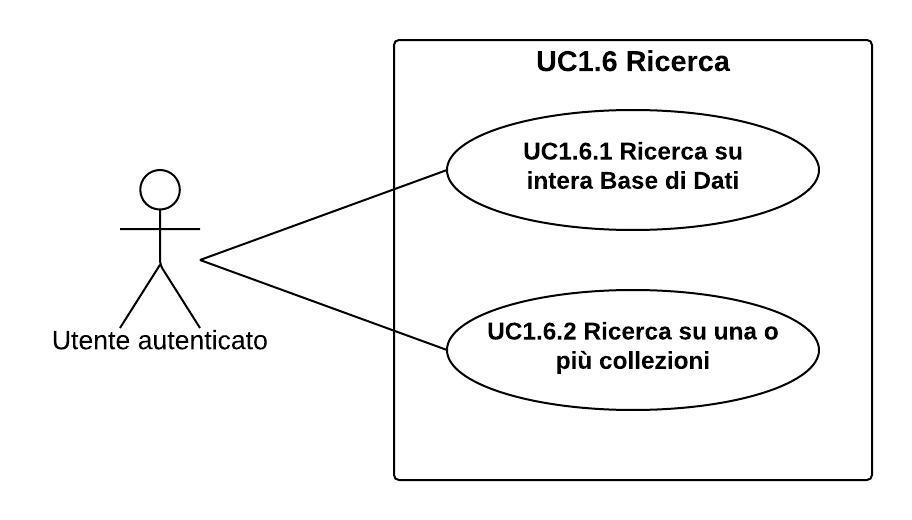
\includegraphics[width=0.7\textwidth,keepaspectratio]{UseCases/UC1_6.jpeg}
    \caption{Caso d'uso 1.6: Ricerca generale}
  \end{center}
\end{figure}
\textbf{Attore primario:} Utente autenticato \\ \\
\textbf{Scopo e descrizione:} L’utente intende effettuare una ricerca, può decidere se effettuare la ricerca su tutte le \gloss{collezioni} di cui ha visibilità o solo su una lista ristretta di esse.\\ \\
\textbf{Precondizione:} Il \gloss{database} è pronto a ricevere comandi e l’utente intende effettuare una ricerca.\\ \\
\textbf{Flusso di eventi:}
\begin{itemize}
\item UC1.6.1 Ricerca sull'intera base di dati;
\item UC1.6.2 Ricerca su una o più \gloss{collezioni}.
\end{itemize}
\begin{itemize}
\item Nel caso in cui l'utente utilizzi un comando sconosciuto:
  \begin{itemize}
  \item viene visualizzato un messaggio di errore esplicativo (e rimando all'aiuto);
  \end{itemize}
\item Nel caso in cui l'utente utilizzi un comando conosciuto ma con parametri errati:
  \begin{itemize}
  \item viene visualizzato un messaggio di supporto che indica come usare correttamente il comando.
  \end{itemize}
\item Nel caso in cui una \gloss{collezione} su cui effettuare ricerca non sia presente:
  \begin{itemize}
  \item viene visualizzato un messaggio di errore esplicativo;
  \end{itemize}
\end{itemize}
\textbf{Postcondizione:} Il sistema ha prodotto in output i risultati della ricerca effettuata.
\subsection{UC1.6.1: Ricerca all'interno della base di dati}
\textbf{Attore primario:} Utente autenticato \\ \\
\textbf{Scopo e descrizione:} L’utente intende effettuare una ricerca sull’intera base di dati a lui visibile, deve inserire i parametri di ricerca.\\ \\
\textbf{Precondizione:} Il \gloss{database} è pronto a ricevere comandi e l’utente intende effettuare una ricerca generale\\ \\
\textbf{Flusso di eventi:}
\begin{itemize}
\item Inserimento parametri di ricerca.
\end{itemize}
\textbf{Postcondizione:} Il sistema ha prodotto in output i risultati della ricerca effettuata.
\subsection{UC1.6.2: Ricerca all'interno di una specifica collezione(o più)}
\textbf{Attore primario:} Utente autenticato \\ \\
\textbf{Scopo e descrizione:} L’utente intende effettuare una ricerca all’interno di una o più \gloss{collezioni} specifiche, deve inserire le \gloss{collezioni} su cui effettuare la ricerca e i parametri di ricerca.\\ \\
\textbf{Precondizione:} Il \gloss{database} è pronto a ricevere comandi e l’utente intende effettuare una ricerca dettagliata\\ \\
\textbf{Flusso di eventi:}
\begin{itemize}
\item Inserimento nomi \gloss{collezioni};
\item Inserimento parametri di ricerca.
\end{itemize}
\textbf{Postcondizione:} Il sistema ha prodotto in output i risultati della ricerca effettuata.
\subsection{UC1.7: Gestione account}
\begin{figure}[H]
  \begin{center}
    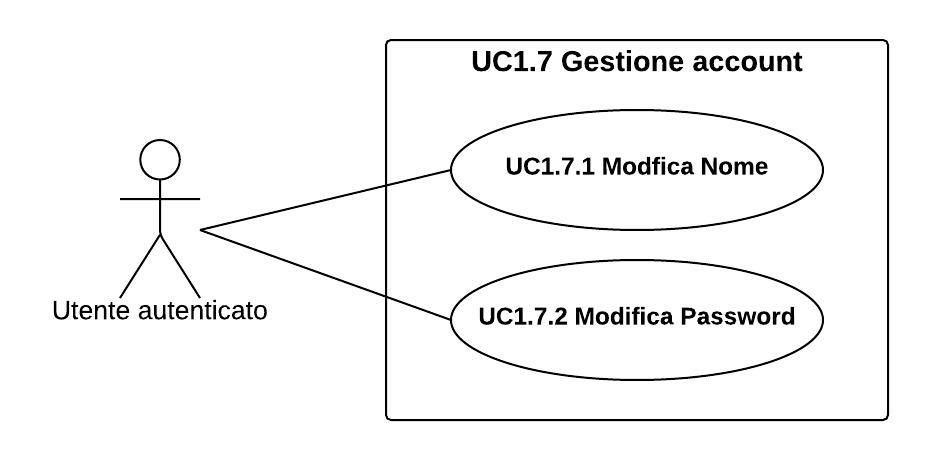
\includegraphics[width=0.7\textwidth,keepaspectratio]{UseCases/UC1_7.jpeg}
    \caption{Caso d'uso 1.7: Gestione \gloss{account}}
  \end{center}
\end{figure}
\textbf{Attore primario:} Utente autenticato\\ \\
\textbf{Scopo e descrizione:} L'utente intende effettuare operazioni di gestione sul proprio \gloss{account}. Le operazioni previste sono
modifica di username e di password.\\ \\
\textbf{Precondizione:} Il \gloss{database} è pronto a ricevere comandi e l'utente intende effettuare operazioni di gestione del proprio \gloss{account}.\\ \\
\textbf{Flusso di eventi:}
\begin{itemize}
\item UC1.7.1 Modifica username;
\item UC1.7.2 Modifica password.
\end{itemize}
\textbf{Estensioni:}
\begin{itemize}
\item Nel caso in cui l'utente utilizzi un comando sconosciuto:
  \begin{itemize}
  \item viene visualizzato un messaggio di errore esplicativo (e rimando all'aiuto);
  \end{itemize}
\item Nel caso in cui l'utente utilizzi un comando conosciuto ma con parametri errati:
  \begin{itemize}
  \item viene visualizzato un messaggio di supporto che indica come usare correttamente il comando.
  \end{itemize}
\item Nel caso in cui il nuovo username scelto sia già presente nel sistema \textbf{Actorbase}:
  \begin{itemize}
  \item viene visualizzato un messaggio di errore esplicativo;
  \end{itemize}
\end{itemize}
\textbf{Postcondizione:} Il sistema ha eseguito correttamente l'operazione richiesta.
\subsection{UC1.7.1: Modifica username}
\textbf{Attore primario:} Utente autenticato\\ \\
\textbf{Scopo e descrizione:} L'utente intende effettuare la modifica del proprio username nel sistema \textbf{Actorbase}. Dovrà inserire il nuovo username.\\ \\
\textbf{Precondizione:} Il \gloss{database} è pronto a ricevere comandi e l'utente intende modificare il proprio username.\\
\textbf{Flusso eventi:}
\begin{itemize}
\item Inserimento nuovo username.
\end{itemize}
\textbf{Postcondizione:} L'utente ha aggiornato correttamente il proprio username.
\subsection{UC1.7.2: Modifica password}
\textbf{Attore primario:} Utente autenticato\\ \\
\textbf{Scopo e descrizione:} L'utente intende effettuare la modifica della propria password nel sistema \textbf{Actorbase}. Dovrà inserire la vecchia password e la nuova password.\\ \\
\textbf{Precondizione:} Il \gloss{database} è pronto a ricevere comandi e l'utente intende modificare la propria password.\\
\textbf{Flusso eventi:}
\begin{itemize}
\item Inserimento nuova password.
\end{itemize}
\textbf{Postcondizione:} L'utente ha aggiornato correttamente la propria password.
\subsection{UC1.8: Logout}
\textbf{Attore primario:} Utente autenticato\\ \\
\textbf{Scopo e descrizione:} L'utente intende effettuare il logout dal sistema \textbf{Actorbase}.\\ \\
\textbf{Precondizione:} Il \gloss{database} è pronto a ricevere comandi e l'utente intende effettuare il logout dal sistema.\\ \\
\textbf{Flusso di eventi:}
\begin{itemize}
\item Inserimento comando di logout.
\end{itemize}
\textbf{Estensioni:}
\begin{itemize}
\item Nel caso in cui l'utente utilizzi un comando sconosciuto:
  \begin{itemize}
  \item viene visualizzato un messaggio di errore esplicativo (e rimando all'aiuto);
  \end{itemize}
\end{itemize}
\textbf{Postcondizione:} L'utente è deautenticato dal sistema \textbf{Actorbase}.
\subsection{UC1.9: Gestione utenti}
\begin{figure}[H]
  \begin{center}
    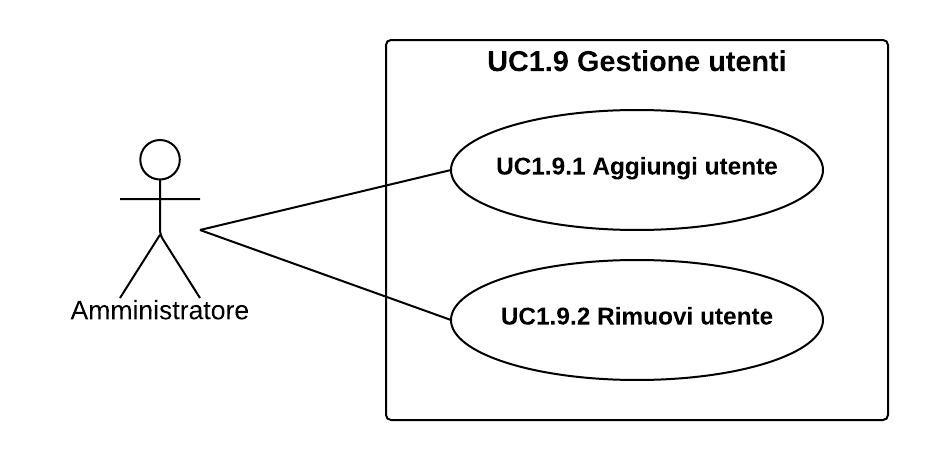
\includegraphics[width=0.7\textwidth,keepaspectratio]{UseCases/UC1_9.jpeg}
    \caption{Caso d'uso 1.9: Gestione utenti}
  \end{center}
\end{figure}
\textbf{Attore primario:} Amministratore\\ \\
\textbf{Scopo e descrizione:} L'amministratore intende effettuare operazioni di gestione sugli utenti del \gloss{database}.\\ \\
\textbf{Precondizione:} Il \gloss{database} è pronto a ricevere comandi e l'amministratore intende effettuare operazioni di gestione sugli utenti del sistema.\\ \\
\textbf{Flusso di eventi:}
\begin{itemize}
\item UC1.9.1: Aggiunta nuovo utente;
\item UC1.9.2: Rimozione utente esistente;
\item UC1.9.3: Concessione permessi a utente;
\item UC1.9.4: Revoca permessi a utente.
\end{itemize}
\textbf{Estensioni:}
\begin{itemize}
\item Nel caso in cui l'amministratore utilizzi un comando sconosciuto:
  \begin{itemize}
  \item viene visualizzato un messaggio di errore esplicativo (e rimando all'aiuto).
  \end{itemize}
\item Nel caso in cui l'amministratore utilizzi un comando conosciuto ma con parametri errati:
  \begin{itemize}
  \item viene visualizzato un messaggio di supporto che indica come usare correttamente il comando.
  \end{itemize}
\item Nel caso in cui lo username scelto sia già presente nel sistema \textbf{Actorbase}:
  \begin{itemize}
  \item viene visualizzato un messaggio di errore esplicativo.
  \end{itemize}
\item Nel caso in cui l'utente designato per la rimozione non sia presente nel sistema \textbf{Actorbase}:
  \begin{itemize}
  \item viene visualizzato un messaggio di errore esplicativo.
  \end{itemize}
\item Nel caso in cui l'utente designato per la concessione o revoca dei permessi non sia presente nel sistema \textbf{Actorbase}:
  \begin{itemize}
  \item viene visualizzato un messaggio di errore esplicativo.
  \end{itemize}
\end{itemize}
\textbf{Postcondizione:} L'operazione di gestione richiesta è andata a buon fine.
\subsection{UC1.9.1: Aggiunta nuovo utente}
\textbf{Attore primario:} Amministratore\\ \\
\textbf{Scopo e descrizione:} L'amministratore intende aggiungere un nuovo utente al sistema \textbf{Actorbase}.\\ \\
\textbf{Precondizione:} Il \gloss{database} è pronto a ricevere comandi e l'amministratore intende aggiungere un nuovo utente al sistema.\\ \\
\textbf{Flusso di eventi:}
\begin{itemize}
\item Inserimento username nuovo utente;
\item Inserimento password nuovo utente.
\end{itemize}
\textbf{Postcondizione:} Il nuovo utente designato per l'aggiunta è presente all'interno del sistema \textbf{Actorbase}.
\subsection{UC1.9.1: Rimozione utente esistente}
\textbf{Attore primario:} Amministratore\\ \\
\textbf{Scopo e descrizione:} L'amministratore intende rimuovere un utente esistente dal sistema \textbf{Actorbase}.\\ \\
\textbf{Precondizione:} Il \gloss{database} è pronto a ricevere comandi e l'amministratore intende rimuovere un utente esistente dal sistema.\\ \\
\textbf{Flusso di eventi:}
\begin{itemize}
\item Inserimento username utente.
\end{itemize}
\textbf{Postcondizione:} L'utente designato per la rimozione non è presente all'interno del sistema \textbf{Actorbase}.
\subsection{UC1.9.2: Concessione permessi a utente}
\textbf{Attore primario:} Amministratore\\ \\
\textbf{Scopo e descrizione:} L'amministratore intende concedere permessi ad un utente esistente.\\ \\
\textbf{Precondizione:} Il \gloss{database} è pronto a ricevere comandi e l'amministratore intende concedere permessi ad un utente esistente nel sistema locale \textbf{Actorbase}.
\textbf{Flusso di eventi:}
\begin{itemize}
\item Inserimento username utente.
\end{itemize}
\textbf{Postcondizione:} L'utente designato ha ricevuto i permessi dall'amministratore.
\subsection{UC1.9.3: Revoca permessi a utente}
\textbf{Attore primario:} Amministratore\\ \\
\textbf{Scopo e descrizione:} L'amministratore intende revocare permessi ad un utente esistente.\\ \\
\textbf{Precondizione:} Il \gloss{database} è pronto a ricevere comandi e l'amministratore intende revocare permessi ad un utente esistente nel sistema locale \textbf{Actorbase}.
\textbf{Flusso di eventi:}
\begin{itemize}
\item Inserimento username utente.
\end{itemize}
\textbf{Postcondizione:} All'utente designato sono stati revocati i permessi dall'amministratore.
\subsection{UC1.10: Visualizzazione errore}
\begin{figure}[H]
  \begin{center}
    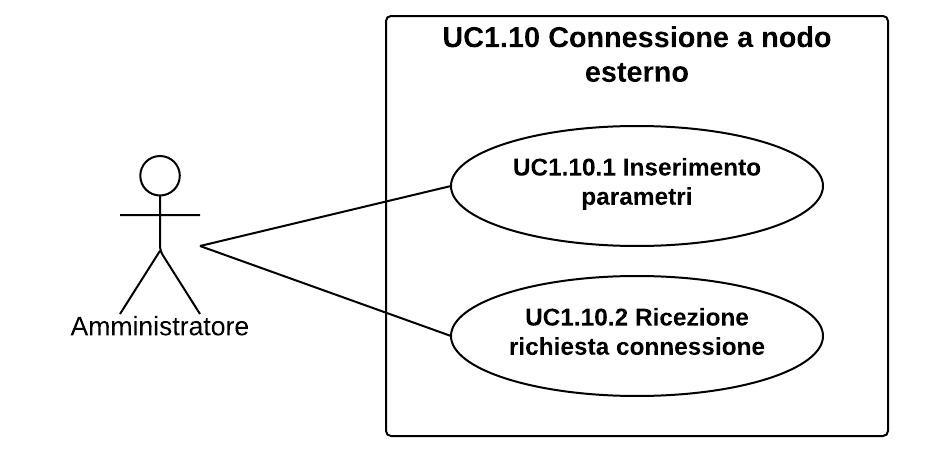
\includegraphics[width=0.7\textwidth,keepaspectratio]{UseCases/UC1_10.jpeg}
    \caption{Caso d'uso 1.10: Visualizzazione errore}
  \end{center}
\end{figure}
\textbf{Attore primario:} Utente \\ \\
\textbf{Scopo e descrizione:} L'utente ha inserito un comando errato o ha effettuato un operazione non permessa. Viene visualizzato un messaggio di errore esplicativo specifico, contestualizzato al caso di errore.\\ \\
\textbf{Precondizione:} L'utente ha inserito un comando errato o ha provato ad effettuare un operazione non permessa.\\ \\
\textbf{Flusso di eventi:}
\begin{itemize}
\item UC1.10.1 Errore scrittura comando;
\item UC1.10.2 Errore di timeout;
\item UC1.10.3 Errore di contesto.
\end{itemize}
\textbf{Postcondizione:} Il sistema ha prodotto in output il messaggio di errore, l'operazione che lo ha generato è stata annullata.
\subsection{UC1.10.1: Errore di scrittura comando}
\textbf{Attore primario:} Utente \\ \\
\textbf{Scopo e descrizione:} L'utente ha inserito un comando errato, il sistema non riconosce il comando.\\ \\
\textbf{Precondizione:} L'utente ha inserito un comando errato.\\ \\
\textbf{Flusso di eventi:}
\begin{itemize}
\item Il sistema non riconosce il comando inserito;
\item Non viene fatta nessuna operazione;
\item Viene visualizzato il messaggio di errore.
\end{itemize}
\textbf{Postcondizione:} Il sistema ha prodotto in output il messaggio di errore, l'operazione che lo ha generato è stata annullata.
\subsection{UC1.10.2: Errore di timeout}
\textbf{Attore primario:} Utente \\ \\
\textbf{Scopo e descrizione:} L'utente ha inserito un comando, il tempo di risposta da parte del sistema ha superato una soglia prefissata.\\ \\
\textbf{Precondizione:} L'operazione richiesta dall'utente sta richiedendo un tempo di risposta troppo elevato.\\ \\
\textbf{Flusso di eventi:}
\begin{itemize}
\item L'operazione supera il tempo di timeout;
\item L'operazione viene annullata;
\item Viene visualizzato il messaggio di errore di timeout.
\end{itemize}
\textbf{Postcondizione:} Il sistema ha prodotto in output il messaggio di errore, l'operazione che lo ha generato è stata annullata.
\subsection{UC1.10.3: Errore di contesto}
\textbf{Attore primario:} Utente \\ \\
\textbf{Scopo e descrizione:} L'utente ha tentato un operazione non permessa o impossibile da soddisfare.\\ \\
\textbf{Precondizione:} L'utente ha tentato un'operazione non permessa o impossibile da soddisfare.\\ \\
\textbf{Flusso di eventi:}
\begin{itemize}
\item Il sistema riconosce che il comando inserito non è consentito;
\item L'operazione viene annullata;
\item Viene visualizzato il messaggio di errore.
\end{itemize}
\textbf{Postcondizione:} Il sistema ha prodotto in output il messaggio di errore di contesto, l'operazione che lo ha generato è stata annullata.
\subsection{UC2: Driver - Interazioni}
\begin{figure}[H]
  \begin{center}
    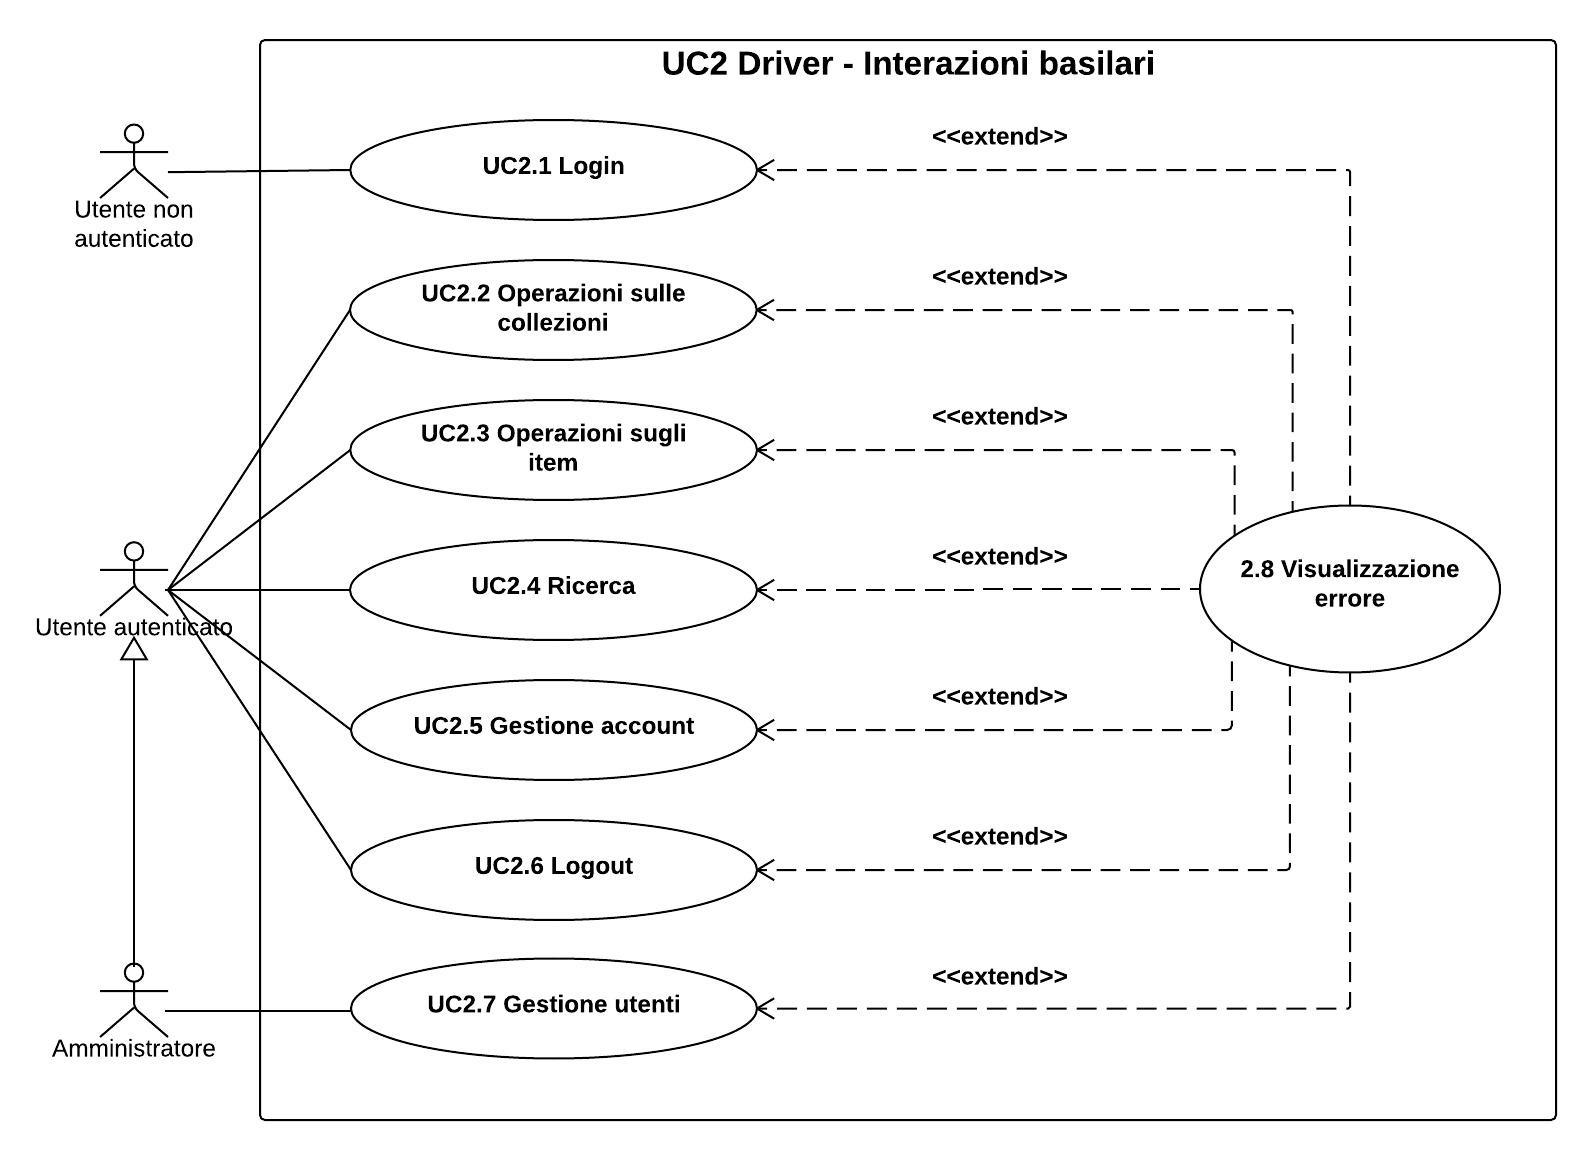
\includegraphics[width=0.7\textwidth,keepaspectratio]{UseCases/UC2.jpeg}
    \caption{Caso d'uso 2: \gloss{Driver} interazioni}
  \end{center}
\end{figure}
\textbf{Attori primari:} Utente non autenticato, Utente autenticato, Amministratore\\ \\
\textbf{Scopo e descrizione:}
L’utente ha appena avviato la \gloss{CLI}, risulta essere non autenticato, può quindi
registrarsi, oppure, se è già registrato, può effettuare il login diventando utente
autenticato. Le operazioni che può eseguire a login effettuato sono:
\begin{itemize}
\item Gestire il proprio \gloss{account};
\item Operazioni sulle \gloss{collezioni};
\item Operazioni sugli \gloss{item};
\item Ricerca;
\item Effettuare il logout.
\end{itemize}
Nel caso in cui si tratti di un amministratore, oltre alle operazioni elencate, può effettuare operazioni di gestione sugli utenti
esistenti nel \gloss{database}.\\ \\
\textbf{Precondizione:} Il \gloss{database} è installato correttamente, e il server è in ascolto.\\ \\
\textbf{Flusso eventi:}
\begin{itemize}
\item UC2.1 Login;
\item UC2.2 Operazioni sulle \gloss{collezione};
\item UC2.3 Operazioni sugli \gloss{item};
\item UC2.4 Ricerca;
\item UC2.5 Gestione \gloss{account};
\item UC2.6 Effettuare il logout;
\item UC2.7 Gestione utenti.
\end{itemize}
\textbf{Postcondizione:} Il sistema ha prodotto l'output corrispondente al
comando immesso dall'utente.\\ \\ I sottocasi d'uso derivati da UC2 sono pari
agli omonimi del caso d'uso UC1. Per evitare una ridondanza in questo documento
si è scelto quindi di non scendere più in dettaglio nell'analisi di questo caso
d'uso.
\section{Requisiti}
\subsection{Requisiti funzionali}
La descrizione dei requisiti segue le regole descritte nelle \href{run:../Interni/NormeDiProgetto\_v1.0.0.pdf}{Norme di Progetto}.
\begin{longtable}[H]{|l|p{2cm}|p{6cm}|p{4cm}|}
  \hline
  \textbf{Requisito} & \textbf{Tipologia} & \textbf{Descrizione} & \textbf{Fonti}\\
  \hline
  OBF1 & \multiLineCell{Funzionale\\Obbligatorio} & Il sistema dovrà fornire un Domain Specific Language per comunicare con il \gloss{database} & \multiLineCell{Capitolato\\UC1\\}\\
  \hline
  DEF1.1 & \multiLineCell{Funzionale\\Desiderabile} & Il sistema dovrà fornire un comando di assistenza & \multiLineCell{UC1.3\\UC1.3.1\\UC1.3.2\\}\\
  \hline
  DEF1.1.1 & \multiLineCell{Funzionale\\Desiderabile} & Il sistema dovrà fornire un comando di assistenza generale & \multiLineCell{UC1.3.1\\}\\
  \hline
  DEF1.1.2 & \multiLineCell{Funzionale\\Desiderabile} & Il sistema dovrà fornire un comando di assistenza specifico per un comando desiderato & \multiLineCell{UC1.3.2\\}\\
  \hline
  OBF2 & \multiLineCell{Funzionale\\Obbligatorio} & Il sistema dovrà fornire un meccanismo di autenticazione & \multiLineCell{UC1\\UC1.1\\UC1.2\\VERBALE20160112\\}\\
  \hline
  OBF2.1 & \multiLineCell{Funzionale\\Obbligatorio} & Il sistema dovrà fornire un meccanismo di registrazione & \multiLineCell{UC1.1\\VERBALE20160119\\}\\
  \hline
  OBF2.2 & \multiLineCell{Funzionale\\Obbligatorio} & Il sistema dovrà fornire un meccanismo di login & \multiLineCell{UC1.2\\UC2\\VERBALE20160119\\}\\
  \hline
  OBF3 & \multiLineCell{Funzionale\\Obbligatorio} & Il sistema dovrà fornire un meccanismo di persistenza dei dati su disco & \multiLineCell{Capitolato\\VERBALE20160112\\}\\
  \hline
  OBF4 & \multiLineCell{Funzionale\\Obbligatorio} & Il sistema dovrà fornire la possibilità di eseguire una serie di operazioni sulle \gloss{collezioni} & \multiLineCell{Capitolato\\UC1.4\\UC2\\}\\
  \hline
  OBF4.1 & \multiLineCell{Funzionale\\Obbligatorio} & Il sistema dovrà fornire la possibilità di creare una nuova \gloss{collezione} & \multiLineCell{UC1.4.1\\VERBALE20160112\\}\\
  \hline
  OBF4.1.1 & \multiLineCell{Funzionale\\Opzionale} & Il sistema deve dare la possibilità di scegliere uno schema delle chiavi che definiscono la \gloss{collezione} da creare & \multiLineCell{UC1.4.1\\VERBALE20160112\\VERBALE20160119\\}\\
  \hline
  OBF4.2 & \multiLineCell{Funzionale\\Obbligatorio} & Il sistema dovrà fornire la possibilità di elencare le \gloss{collezioni} presenti all'interno & \multiLineCell{UC1.4.3\\UC2\\VERBALE20160112\\}\\
  \hline
  OBF4.3 & \multiLineCell{Funzionale\\Obbligatorio} & Il sistema dovrà fornire la possibilità di cancellare una o più \gloss{collezioni} & \multiLineCell{UC1.4.3\\UC2\\VERBALE20160112\\}\\
  \hline
  OBF4.4 & \multiLineCell{Funzionale\\Obbligatorio} & Il sistema dovrà fornire la possibilità di modificare il nome delle \gloss{collezioni} & \multiLineCell{UC1.4.4\\UC2\\VERBALE20160112\\}\\
  \hline
  OBF4.5 & \multiLineCell{Funzionale\\Obbligatorio} & Il sistema dovrà fornire la possibilità di aggiungere collaboratori ad una propria \gloss{collezione} & \multiLineCell{UC1.4.5\\UC2\\VERBALE20160112\\}\\
  \hline
  OBF4.6 & \multiLineCell{Funzionale\\Obbligatorio} & Il sistema dovrà fornire la possibilità di rimuovere un collaboratore da una propria \gloss{collezione} & \multiLineCell{UC1.4.6\\UC2\\VERBALE20160112\\}\\
  \hline
  OBF5 & \multiLineCell{Funzionale\\Obbligatorio} & Il sistema dovrà fornire la possibilità di eseguire una serie di operazioni sugli \gloss{item} & \multiLineCell{Capitolato\\UC1.5\\UC1.5.1\\UC1.5.1.1\\UC1.5.1.2\\UC1.5.2\\UC2\\VERBALE20160112\\}\\
  \hline
  OBF5.1 & \multiLineCell{Funzionale\\Obbligatorio} & Il sistema dovrà permettere l'inserimento di nuovi \gloss{item} & \multiLineCell{Capitolato\\UC1.5.1\\UC2\\VERBALE20160112\\}\\
  \hline
  OBF5.1.1 & \multiLineCell{Funzionale\\Obbligatorio} & Il sistema dovrà permettere la sovrascrittura di un \gloss{item} attraverso inserimento & \multiLineCell{Capitolato\\UC1.5.1.1\\UC2\\VERBALE20160112\\}\\
  \hline
  OBF5.1.2 & \multiLineCell{Funzionale\\Obbligatorio} & Il sistema dovrà permettere l'aggiunta di un nuovo \gloss{item} senza eseguire sovrascrittura & \multiLineCell{Capitolato\\UC1.5.1.2\\UC2\\VERBALE20160112\\}\\
  \hline
  OBF5.2 & \multiLineCell{Funzionale\\Obbligatorio} & Il sistema dovrà permettere la cancellazione di un \gloss{item} & \multiLineCell{Capitolato\\UC1.5.2\\VERBALE20160112\\}\\
  \hline
  DEF5.3 & \multiLineCell{Funzionale\\Desiderabile} & Il sistema dovrà permettere tutte le operazioni sugli \gloss{item} anche attraverso importazione di \gloss{file} & \multiLineCell{UC1.5\\UC1.5.1\\UC1.5.1.1\\UC1.5.1.2\\UC1.5.2\\VERBALE20160112\\}\\
  \hline
  OBF6 & \multiLineCell{Funzionale\\Obbligatorio} & Il sistema dovrà fornire un meccanismo di ricerca & \multiLineCell{UC1.6\\UC2\\VERBALE20160112\\}\\
  \hline
  OBF6.1 & \multiLineCell{Funzionale\\Obbligatorio} & Il sistema dovrà fornire un meccanismo di ricerca generale sull'intera base di dati & \multiLineCell{UC1.6.1\\UC2\\VERBALE20160112\\}\\
  \hline
  OBF6.2 & \multiLineCell{Funzionale\\Obbligatorio} & Il sistema dovrà fornire la possibilità di effettuare ricerche su una o più \gloss{collezioni} & \multiLineCell{UC1.6.2\\UC2\\VERBALE20160112\\}\\
  \hline
  OBF7 & \multiLineCell{Funzionale\\Obbligatorio} & Il sistema dovrà fornire un meccanismo per la gestione del proprio \gloss{account} & \multiLineCell{UC1.7\\UC1.7.1\\UC1.7.2\\VERBALE20160112\\}\\
  \hline
  DEF7.1 & \multiLineCell{Funzionale\\Desiderabile} & Il sistema dovrà fornire la possibilità di cambiare il proprio username & \multiLineCell{UC1.7\\UC1.7.1\\VERBALE20160112\\}\\
  \hline
  OBF7.2 & \multiLineCell{Funzionale\\Obbligatorio} & Il sistema dovrà fornire la possibilità di cambiare la propria password & \multiLineCell{UC1.7\\UC1.7.2\\VERBALE20160112\\}\\
  \hline
  OBF8 & \multiLineCell{Funzionale\\Obbligatorio} & Il sistema dovrà permettere di effettuare logout & \multiLineCell{UC1.8\\VERBALE20160112\\}\\
  \hline
  DEF9 & \multiLineCell{Funzionale\\Desiderabile} & Il sistema dovrà fornire diverse azioni possibili sugli \gloss{account} agli amministratori & \multiLineCell{UC1.9\\UC1.9.1\\UC1.9.2\\UC2\\}\\
  \hline
  DEF9.1 & \multiLineCell{Funzionale\\Desiderabile} & Il sistema dovrà permettere agli amministratori di aggiungere nuovi utenti & \multiLineCell{UC1.9\\UC1.9.1\\UC2\\}\\
  \hline
  DEF9.2 & \multiLineCell{Funzionale\\Desiderabile} & Il sistema dovrà permettere agli amministratori di eliminare utenti esistenti & \multiLineCell{UC1.9\\UC1.9.2\\UC2\\}\\
  \hline
  OBF10 & \multiLineCell{Funzionale\\Obbligatorio} & Il sistema dovrà fornire un meccanismo di connessione ad altre istanze esterne & \multiLineCell{Capitolato\\UC1\\VERBALE20160112\\VERBALE20160119\\}\\
  \hline
  OBF11 & \multiLineCell{Funzionale\\Obbligatorio} & Il sistema dovrà permettere la visualizzazione di un messaggio di errore & \multiLineCell{UC1.10\\UC1.10.1\\UC1.10.2\\VERBALE20160112\\}\\
  \hline
  OBF11.1 & \multiLineCell{Funzionale\\Obbligatorio} & Il sistema dovrà permettere la visualizzazione di un messaggio di errore in caso di inserimenti di un comando errato & \multiLineCell{UC1.10\\UC1.10.1\\VERBALE20160112\\}\\
  \hline
  OBF11.2 & \multiLineCell{Funzionale\\Obbligatorio} & Il sistema dovrà permettere la visualizzazione di un messaggio d'errore in caso di timeout & \multiLineCell{UC1.10.2\\VERBALE20160112\\}\\
  \hline
  OBF11.3 & \multiLineCell{Funzionale\\Obbligatorio} & Il sistema dovrà permettere la visualizzazione di un messaggio di errore qualora si tenti di eseguire una operazione non permessa o impossibile da soddisfare & \multiLineCell{UC1.11.3\\VERBALE20160112\\}\\
  \hline
  DEF12 & \multiLineCell{Funzionale\\Desiderabile} & Dovrà essere fornito un \gloss{driver} Scala per interfacciarsi ad Actorbase & \multiLineCell{Capitolato\\UC2\\VERBALE20160112\\}\\
  \hline
  DEF12.1 & \multiLineCell{Funzionale\\Desiderabile} & Il \gloss{driver} dovrà permettere di effettuare il login & \multiLineCell{UC2\\}\\
  \hline
  DEF12.10 & \multiLineCell{Funzionale\\Desiderabile} & Il \gloss{driver} dovrà permettere la ricerca all'interno di \gloss{collezioni} & \multiLineCell{UC2\\}\\
  \hline
  DEF12.11 & \multiLineCell{Funzionale\\Desiderabile} & Il \gloss{driver} dovrà permettere il logout dal \gloss{database} & \multiLineCell{UC2\\}\\
  \hline
  DEF12.2 & \multiLineCell{Funzionale\\Desiderabile} & Il \gloss{driver} dovrà permettere la creazione di \gloss{collezioni} & \multiLineCell{UC2\\}\\
  \hline
  DEF12.3 & \multiLineCell{Funzionale\\Desiderabile} & Il \gloss{driver} dovrà permettere l'elencazione delle \gloss{collezioni} & \multiLineCell{UC2\\}\\
  \hline
  DEF12.4 & \multiLineCell{Funzionale\\Desiderabile} & Il \gloss{driver} dovrà permettere la modifica del nome di una \gloss{collezione} & \multiLineCell{UC2\\}\\
  \hline
  DEF12.5 & \multiLineCell{Funzionale\\Desiderabile} & Il \gloss{driver} dovrà permettere l'aggiunta di un collaboratore al \gloss{collezione} & \multiLineCell{UC2\\}\\
  \hline
  DEF12.6 & \multiLineCell{Funzionale\\Desiderabile} & Il \gloss{driver} dovrà permetter la rimozione di un collaboratore dalle \gloss{collezioni} & \multiLineCell{UC2\\}\\
  \hline
  DEF12.7 & \multiLineCell{Funzionale\\Desiderabile} & Il \gloss{driver} dovrà permettere l'inserimento di \gloss{item} nelle \gloss{collezioni} & \multiLineCell{UC2\\}\\
  \hline
  DEF12.7.1 & \multiLineCell{Funzionale\\Desiderabile} & Il \gloss{driver} dovrà permettere l'inserimento \gloss{item} con sovrascrittura nelle \gloss{collezioni} & \multiLineCell{UC2\\}\\
  \hline
  DEF12.7.2 & \multiLineCell{Funzionale\\Desiderabile} & Il \gloss{driver} dovrà permettere l'inserimento senza sovrascrittura nelle \gloss{collezioni} & \multiLineCell{UC2\\}\\
  \hline
  DEF12.8 & \multiLineCell{Funzionale\\Desiderabile} & Il \gloss{driver} dovrà permettere la cancellazione di \gloss{item} dalle \gloss{collezioni} & \multiLineCell{UC2\\}\\
  \hline
  DEF12.9 & \multiLineCell{Funzionale\\Desiderabile} & Il \gloss{driver} dovrà permettere la ricerca all'interno del \gloss{database} & \multiLineCell{UC2\\}\\
  \hline
  OBF19 & \multiLineCell{Funzionale\\Obbligatorio} & Sarà implementato l'\gloss{attore} di tipo \gloss{storekeeper} & \multiLineCell{Capitolato\\}\\
  \hline
  OBF19.1 & \multiLineCell{Funzionale\\Obbligatorio} & Gli \gloss{attori} di tipo \gloss{storekeeper} dovranno contenere le diverse coppie chiave/valore & \multiLineCell{Capitolato\\}\\
  \hline
  OBF19.2 & \multiLineCell{Funzionale\\Obbligatorio} & Gli \gloss{storekeeper} dovranno soddisfare le richieste provenienti dai rispettivi \gloss{storefinder} & \multiLineCell{Capitolato\\}\\
  \hline
  OBF20 & \multiLineCell{Funzionale\\Obbligatorio} & Sarà implementato l'\gloss{attore} di tipo \gloss{storefinder} & \multiLineCell{Capitolato\\}\\
  \hline
  OBF20.1 & \multiLineCell{Funzionale\\Obbligatorio} & Gli \gloss{attori} \gloss{storefinder} possono ricevere richieste dall'esterno & \multiLineCell{Capitolato\\}\\
  \hline
  OBF20.2 & \multiLineCell{Funzionale\\Obbligatorio} & Gli \gloss{attori} di tipo \gloss{storefinder} dovranno instradare le richieste ai giusti \gloss{storekeeper} & \multiLineCell{Capitolato\\}\\
  \hline
  OBF21 & \multiLineCell{Funzionale\\Obbligatorio} & Sarà implementato l'\gloss{attore} di tipo \gloss{warehousemen} & \multiLineCell{Capitolato\\}\\
  \hline
  OBF21.1 & \multiLineCell{Funzionale\\Obbligatorio} & Il sistema dovrà permettere agli \gloss{attori} \gloss{warehousemen} di mandare messaggi agli \gloss{attori} di tipo \gloss{storekeeper} & \multiLineCell{Capitolato\\}\\
  \hline
  OBF21.2 & \multiLineCell{Funzionale\\Obbligatorio} & Il sistema dovrà permettere agli \gloss{attori} \gloss{warehousemen} di ricevere messaggi dagli \gloss{attori} di tipo \gloss{storekeeper} & \multiLineCell{Capitolato\\}\\
  \hline
  OBF21.3 & \multiLineCell{Funzionale\\Obbligatorio} & Il sistema dovrà permettere agli \gloss{attori} \gloss{warehousemen} di persistere i dati su disco & \multiLineCell{Capitolato\\}\\
  \hline
  OPF22 & \multiLineCell{Funzionale\\Opzionale} & Sarà implementato l'\gloss{attore} di tipo ninja & \multiLineCell{Capitolato\\}\\
  \hline
  OPF22.1 & \multiLineCell{Funzionale\\Opzionale} & L'\gloss{attore} di tipo ninja dovrà poter essere eletto a \gloss{storekeeper} se necessario & \multiLineCell{Capitolato\\}\\
  \hline
  OPF22.2 & \multiLineCell{Funzionale\\Opzionale} & L'\gloss{attore} di tipo ninja dovrà essere aggiornato insieme al corrispondente \gloss{storekeeper} & \multiLineCell{Capitolato\\}\\
  \hline
  OPF23 & \multiLineCell{Funzionale\\Opzionale} & Sarà implementato l'\gloss{attore} di tipo manager & \multiLineCell{Capitolato\\}\\
  \hline
  OPF23.1 & \multiLineCell{Funzionale\\Opzionale} & L'\gloss{attore} manager dovrà decidere il numero massimo di \gloss{item} contenuti in un'istanza dello \gloss{storekeeper} & \multiLineCell{Capitolato\\}\\
  \hline
  OPF23.1.1 & \multiLineCell{Funzionale\\Opzionale} & L'\gloss{attore} manager dovrà decidere il numero massimo di \gloss{item} contenuti in un istanza di \gloss{storekeeper} in maniera statica & \multiLineCell{Capitolato\\}\\
  \hline
  OPF23.1.2 & \multiLineCell{Funzionale\\Opzionale} & L'\gloss{attore} manager dovrà decidere il numero massimo di \gloss{item} contenuti in un istanza di \gloss{storekeeper} in maniera dinamica in base al carico & \multiLineCell{Capitolato\\}\\
  \hline
  OPF23.2 & \multiLineCell{Funzionale\\Opzionale} & L'\gloss{attore} manager dovrà poter inviare e ricevere messaggi agli \gloss{storekeeper} & \multiLineCell{Capitolato\\}\\
  \hline
  OBF24 & \multiLineCell{Funzionale\\Obbligatorio} & Sarà implementato l'\gloss{attore} di tipo main & \multiLineCell{Capitolato\\}\\
  \hline
  OBF26 & \multiLineCell{Funzionale\\Obbligatorio} & Il sistema dovrà distinguere diversi tipi di \gloss{account}. Utente non autenticato, utente autenticato e utente amministratore & \multiLineCell{UC1\\UC1.1\\UC1.2\\UC1.7\\UC1.7.1\\UC1.7.2\\UC1.8\\UC1.9\\UC1.9.1\\UC1.9.2\\VERBALE20160112\\}\\
  \hline
\end{longtable}
\subsection{Requisiti di vincolo}
\begin{longtable}[H]{|l|p{2cm}|p{6cm}|p{4cm}|}
  \hline
  \textbf{Requisito} & \textbf{Tipologia} & \textbf{Descrizione} & \textbf{Fonti}\\
  \hline
  OBV13 & \multiLineCell{Vincolo\\Obbligatorio} & Il sistema dovrà funzionare in ambienti Ubuntu 14.04 o superiore & \multiLineCell{VERBALE20160119\\}\\
  \hline
  OBV14 & \multiLineCell{Vincolo\\Obbligatorio} & Il sistema dovrà funzionare su \gloss{JVM} & \multiLineCell{Capitolato\\}\\
  \hline
  DEV15 & \multiLineCell{Vincolo\\Desiderabile} & Il sistema dovrà funzionare in ambienti Windows 10 o superiori & \multiLineCell{VERBALE20160119\\}\\
  \hline
  DEV16 & \multiLineCell{Vincolo\\Desiderabile} & Il sistema dovrà funzionare su sistemi OSX el capitan o superiori & \multiLineCell{VERBALE20160119\\}\\
  \hline
  OBV25 & \multiLineCell{Vincolo\\Obbligatorio} & Il sistema dovrà utilizzare la libreria Akka & \multiLineCell{Capitolato\\}\\
  \hline
\end{longtable}
\subsection{Requisiti di qualità}
\begin{longtable}[H]{|l|p{2cm}|p{6cm}|p{4cm}|}
  \hline
  \textbf{Requisito} & \textbf{Tipologia} & \textbf{Descrizione} & \textbf{Fonti}\\
  \hline
  OBQ17 & \multiLineCell{Qualitativo\\Obbligatorio} & Dovrà essere fornito un manuale utente redatto in lingua inglese & \multiLineCell{Capitolato\\}\\
  \hline
  OBF18 & \multiLineCell{Qualitativo\\Obbligatorio} & Dovranno essere rispettate tutte le norme e le metriche sulla stesura del codice come riportato nelle \textit{Norme di Progetto} & \multiLineCell{INTERNO\\}\\
  \hline
  OBQ18.1 & \multiLineCell{Qualitativo\\Obbligatorio} & Dovrà essere prodotta documentazione in Scaladoc del prodotto & \multiLineCell{NORME\\}\\
  \hline
\end{longtable}
\section{Tracciamento Requisiti-Fonti}
\begin{longtable}[H]{|p{5.5cm}|p{5.5cm}|}
  \hline
  \textbf{Requisito} & \textbf{Fonti}\\
  \hline
  OBF1 & \multiLineCell[t]{Capitolato\\UC1\\}\\
  \hline
  DEF1.1 & \multiLineCell[t]{UC1.3\\UC1.3.1\\UC1.3.2\\}\\
  \hline
  DEF1.1.1 & \multiLineCell[t]{UC1.3.1\\}\\
  \hline
  DEF1.1.2 & \multiLineCell[t]{UC1.3.2\\}\\
  \hline
  OBF2 & \multiLineCell[t]{UC1\\UC1.1\\UC1.2\\VERBALE20160112\\}\\
  \hline
  OBF2.1 & \multiLineCell[t]{UC1.1\\VERBALE20160119\\}\\
  \hline
  OBF2.2 & \multiLineCell[t]{UC1.2\\UC2\\VERBALE20160119\\}\\
  \hline
  OBF3 & \multiLineCell[t]{Capitolato\\VERBALE20160112\\}\\
  \hline
  OBF4 & \multiLineCell[t]{Capitolato\\UC1.4\\UC2\\}\\
  \hline
  OBF4.1 & \multiLineCell[t]{UC1.4.1\\VERBALE20160112\\}\\
  \hline
  OBF4.1.1 & \multiLineCell[t]{UC1.4.1\\VERBALE20160112\\VERBALE20160119\\}\\
  \hline
  OBF4.2 & \multiLineCell[t]{UC1.4.3\\UC2\\VERBALE20160112\\}\\
  \hline
  OBF4.3 & \multiLineCell[t]{UC1.4.3\\UC2\\VERBALE20160112\\}\\
  \hline
  OBF4.4 & \multiLineCell[t]{UC1.4.4\\UC2\\VERBALE20160112\\}\\
  \hline
  OBF4.5 & \multiLineCell[t]{UC1.4.5\\UC2\\VERBALE20160112\\}\\
  \hline
  OBF4.6 & \multiLineCell[t]{UC1.4.6\\UC2\\VERBALE20160112\\}\\
  \hline
  OBF5 & \multiLineCell[t]{Capitolato\\UC1.5\\UC1.5.1\\UC1.5.1.1\\UC1.5.1.2\\UC1.5.2\\UC2\\VERBALE20160112\\}\\
  \hline
  OBF5.1 & \multiLineCell[t]{Capitolato\\UC1.5.1\\UC2\\VERBALE20160112\\}\\
  \hline
  OBF5.1.1 & \multiLineCell[t]{Capitolato\\UC1.5.1.1\\UC2\\VERBALE20160112\\}\\
  \hline
  OBF5.1.2 & \multiLineCell[t]{Capitolato\\UC1.5.1.2\\UC2\\VERBALE20160112\\}\\
  \hline
  OBF5.2 & \multiLineCell[t]{Capitolato\\UC1.5.2\\VERBALE20160112\\}\\
  \hline
  DEF5.3 & \multiLineCell[t]{UC1.5\\UC1.5.1\\UC1.5.1.1\\UC1.5.1.2\\UC1.5.2\\VERBALE20160112\\}\\
  \hline
  OBF6 & \multiLineCell[t]{UC1.6\\UC2\\VERBALE20160112\\}\\
  \hline
  OBF6.1 & \multiLineCell[t]{UC1.6.1\\UC2\\VERBALE20160112\\}\\
  \hline
  OBF6.2 & \multiLineCell[t]{UC1.6.2\\UC2\\VERBALE20160112\\}\\
  \hline
  OBF7 & \multiLineCell[t]{UC1.7\\UC1.7.1\\UC1.7.2\\VERBALE20160112\\}\\
  \hline
  DEF7.1 & \multiLineCell[t]{UC1.7\\UC1.7.1\\VERBALE20160112\\}\\
  \hline
  OBF7.2 & \multiLineCell[t]{UC1.7\\UC1.7.2\\VERBALE20160112\\}\\
  \hline
  OBF8 & \multiLineCell[t]{UC1.8\\VERBALE20160112\\}\\
  \hline
  DEF9 & \multiLineCell[t]{UC1.9\\UC1.9.1\\UC1.9.2\\UC2\\}\\
  \hline
  DEF9.1 & \multiLineCell[t]{UC1.9\\UC1.9.1\\UC2\\}\\
  \hline
  DEF9.2 & \multiLineCell[t]{UC1.9\\UC1.9.2\\UC2\\}\\
  \hline
  OBF10 & \multiLineCell[t]{Capitolato\\UC1\\VERBALE20160112\\VERBALE20160119\\}\\
  \hline
  OBF11 & \multiLineCell[t]{UC1.10\\UC1.10.1\\UC1.10.2\\VERBALE20160112\\}\\
  \hline
  OBF11.1 & \multiLineCell[t]{UC1.10\\UC1.10.1\\VERBALE20160112\\}\\
  \hline
  OBF11.2 & \multiLineCell[t]{UC1.10.2\\VERBALE20160112\\}\\
  \hline
  OBF11.3 & \multiLineCell[t]{UC1.11.3\\VERBALE20160112\\}\\
  \hline
  DEF12 & \multiLineCell[t]{Capitolato\\UC2\\VERBALE20160112\\}\\
  \hline
  DEF12.1 & \multiLineCell[t]{UC2\\}\\
  \hline
  DEF12.10 & \multiLineCell[t]{UC2\\}\\
  \hline
  DEF12.11 & \multiLineCell[t]{UC2\\}\\
  \hline
  DEF12.2 & \multiLineCell[t]{UC2\\}\\
  \hline
  DEF12.3 & \multiLineCell[t]{UC2\\}\\
  \hline
  DEF12.4 & \multiLineCell[t]{UC2\\}\\
  \hline
  DEF12.5 & \multiLineCell[t]{UC2\\}\\
  \hline
  DEF12.6 & \multiLineCell[t]{UC2\\}\\
  \hline
  DEF12.7 & \multiLineCell[t]{UC2\\}\\
  \hline
  DEF12.7.1 & \multiLineCell[t]{UC2\\}\\
  \hline
  DEF12.7.2 & \multiLineCell[t]{UC2\\}\\
  \hline
  DEF12.8 & \multiLineCell[t]{UC2\\}\\
  \hline
  DEF12.9 & \multiLineCell[t]{UC2\\}\\
  \hline
  OBV13 & \multiLineCell[t]{VERBALE20160119\\}\\
  \hline
  OBV14 & \multiLineCell[t]{Capitolato\\}\\
  \hline
  DEV15 & \multiLineCell[t]{VERBALE20160119\\}\\
  \hline
  DEV16 & \multiLineCell[t]{VERBALE20160119\\}\\
  \hline
  OBQ17 & \multiLineCell[t]{Capitolato\\}\\
  \hline
  OBQ18 & \multiLineCell[t]{INTERNO\\}\\
  \hline
  OBQ18.1 & \multiLineCell[t]{NORME\\}\\
  \hline
  OBF19 & \multiLineCell[t]{Capitolato\\}\\
  \hline
  OBF19.1 & \multiLineCell[t]{Capitolato\\}\\
  \hline
  OBF19.2 & \multiLineCell[t]{Capitolato\\}\\
  \hline
  OBF20 & \multiLineCell[t]{Capitolato\\}\\
  \hline
  OBF20.1 & \multiLineCell[t]{Capitolato\\}\\
  \hline
  OBF20.2 & \multiLineCell[t]{Capitolato\\}\\
  \hline
  OBF21 & \multiLineCell[t]{Capitolato\\}\\
  \hline
  OBF21.1 & \multiLineCell[t]{Capitolato\\}\\
  \hline
  OBF21.2 & \multiLineCell[t]{Capitolato\\}\\
  \hline
  OBF21.3 & \multiLineCell[t]{Capitolato\\}\\
  \hline
  OPF22 & \multiLineCell[t]{Capitolato\\}\\
  \hline
  OPF22.1 & \multiLineCell[t]{Capitolato\\}\\
  \hline
  OPF22.2 & \multiLineCell[t]{Capitolato\\}\\
  \hline
  OPF23 & \multiLineCell[t]{Capitolato\\}\\
  \hline
  OPF23.1 & \multiLineCell[t]{Capitolato\\}\\
  \hline
  OPF23.1.1 & \multiLineCell[t]{Capitolato\\}\\
  \hline
  OPF23.1.2 & \multiLineCell[t]{Capitolato\\}\\
  \hline
  OPF23.2 & \multiLineCell[t]{Capitolato\\}\\
  \hline
  OBF24 & \multiLineCell[t]{Capitolato\\}\\
  \hline
  OBV25 & \multiLineCell[t]{Capitolato\\}\\
  \hline
  OBF26 & \multiLineCell[t]{UC1\\UC1.1\\UC1.2\\UC1.7\\UC1.7.1\\UC1.7.2\\UC1.8\\UC1.9\\UC1.9.1\\UC1.9.2\\VERBALE20160112\\}\\
  \hline
\end{longtable}
\newpage
\section{Tracciamento Fonti-Requisiti}
\begin{longtable}[H]{|p{5.5cm}|p{5.5cm}|}
  \hline
  \textbf{Fonte} & \textbf{Requisiti}\\
  \hline
  Capitolato & \multiLineCell[t]{DEF12\\OBF1\\OBF10\\OBF19\\OBF19.1\\OBF19.2\\OBF20\\OBF20.1\\OBF20.2\\OBF21\\OBF21.1\\OBF21.2\\OBF21.3\\OBF24\\OBF3\\OBF4\\OBF5\\OBF5.1\\OBF5.1.1\\OBF5.1.2\\OBF5.2\\OBQ17\\OBV14\\OBV25\\OPF22\\OPF22.1\\OPF22.2\\OPF23\\OPF23.1\\OPF23.1.1\\OPF23.1.2\\OPF23.2\\}\\
  \hline
  INTERNO & \multiLineCell[t]{OBF18\\}\\
  \hline
  NORME & \multiLineCell[t]{OBQ18\\}\\
  \hline
  UC1 & \multiLineCell[t]{OBF1\\OBF10\\OBF12\\OBF2\\}\\
  \hline
  UC1.1 & \multiLineCell[t]{OBF12\\OBF2\\OBF2.1\\}\\
  \hline
  UC1.10 & \multiLineCell[t]{OBF11\\OBF11.1\\}\\
  \hline
  UC1.10.1 & \multiLineCell[t]{OBF11\\OBF11.1\\}\\
  \hline
  UC1.10.2 & \multiLineCell[t]{OBF11\\OBF11.2\\}\\
  \hline
  UC1.11.3 & \multiLineCell[t]{OBF11.3\\}\\
  \hline
  UC1.2 & \multiLineCell[t]{OBF12\\OBF2\\OBF2.2\\}\\
  \hline
  UC1.3 & \multiLineCell[t]{DEF1.1\\}\\
  \hline
  UC1.3.1 & \multiLineCell[t]{DEF1.1\\DEF1.1.1\\}\\
  \hline
  UC1.3.2 & \multiLineCell[t]{DEF1.1\\DEF1.1.2\\}\\
  \hline
  UC1.4 & \multiLineCell[t]{OBF4\\}\\
  \hline
  UC1.4.1 & \multiLineCell[t]{OBF4.1\\OBF4.1.1\\}\\
  \hline
  UC1.4.3 & \multiLineCell[t]{OBF4.2\\OBF4.3\\}\\
  \hline
  UC1.4.4 & \multiLineCell[t]{OBF4.4\\}\\
  \hline
  UC1.4.5 & \multiLineCell[t]{OBF4.5\\}\\
  \hline
  UC1.4.6 & \multiLineCell[t]{OBF4.6\\}\\
  \hline
  UC1.5 & \multiLineCell[t]{DEF5.3\\OBF5\\}\\
  \hline
  UC1.5.1 & \multiLineCell[t]{DEF5.3\\OBF5\\OBF5.1\\}\\
  \hline
  UC1.5.1.1 & \multiLineCell[t]{DEF5.3\\OBF5\\OBF5.1.1\\}\\
  \hline
  UC1.5.1.2 & \multiLineCell[t]{DEF5.3\\OBF5\\OBF5.1.2\\}\\
  \hline
  UC1.5.2 & \multiLineCell[t]{DEF5.3\\OBF5\\OBF5.2\\}\\
  \hline
  UC1.6 & \multiLineCell[t]{OBF6\\}\\
  \hline
  UC1.6.1 & \multiLineCell[t]{OBF6.1\\}\\
  \hline
  UC1.6.2 & \multiLineCell[t]{OBF6.2\\}\\
  \hline
  UC1.7 & \multiLineCell[t]{DEF7.1\\OBF12\\OBF7\\OBF7.2\\}\\
  \hline
  UC1.7.1 & \multiLineCell[t]{DEF7.1\\OBF12\\OBF7\\}\\
  \hline
  UC1.7.2 & \multiLineCell[t]{OBF12\\OBF7\\OBF7.2\\}\\
  \hline
  UC1.8 & \multiLineCell[t]{OBF12\\OBF8\\}\\
  \hline
  UC1.9 & \multiLineCell[t]{DEF9\\DEF9.1\\DEF9.2\\OBF12\\}\\
  \hline
  UC1.9.1 & \multiLineCell[t]{DEF9\\DEF9.1\\OBF12\\}\\
  \hline
  UC1.9.2 & \multiLineCell[t]{DEF9\\DEF9.2\\OBF12\\}\\
  \hline
  UC2 & \multiLineCell[t]{DEF12\\DEF12.1\\DEF12.10\\DEF12.11\\DEF12.2\\DEF12.3\\DEF12.4\\DEF12.5\\DEF12.6\\DEF12.7\\DEF12.7.1\\DEF12.7.2\\DEF12.8\\DEF12.9\\DEF9\\DEF9.1\\DEF9.2\\OBF2.2\\OBF4\\OBF4.2\\OBF4.3\\OBF4.4\\OBF4.5\\OBF4.6\\OBF5\\OBF5.1\\OBF5.1.1\\OBF5.1.2\\OBF6\\OBF6.1\\OBF6.2\\}\\
  \hline
  VERBALE20160112 & \multiLineCell[t]{DEF12\\DEF5.3\\DEF7.1\\OBF10\\OBF11\\OBF11.1\\OBF11.2\\OBF11.3\\OBF12\\OBF2\\OBF3\\OBF4.1\\OBF4.1.1\\OBF4.2\\OBF4.3\\OBF4.4\\OBF4.5\\OBF4.6\\OBF5\\OBF5.1\\OBF5.1.1\\OBF5.1.2\\OBF5.2\\OBF6\\OBF6.1\\OBF6.2\\OBF7\\OBF7.2\\OBF8\\}\\
  \hline
  VERBALE20160119 & \multiLineCell[t]{DEV15\\DEV16\\OBF10\\OBF2.1\\OBF2.2\\OBF4.1.1\\OBV13\\}\\
  \hline
\end{longtable}
\section{Riepilogo}
\begin{table}[H]
  \centering
  \caption{Riepilogo requisiti}
  \begin{tabular}{|l|l|l|l|}
    \hline
    Categoria & Obbligatorio & Desiderabile & Opzionale\\
    \hline
    Funzionale & 40 & 22 & 9 \\
    \hline
    di Qualità & 3 & 0 & 0 \\
    \hline
    di Vincolo & 3 & 2 & 0 \\
    \hline
  \end{tabular}
\end{table}
\end{document}
